%\documentclass[10pt,twocolumn,twoside]{IEEEtran}
\documentclass[10pt,draftcls,onecolumn]{IEEEtran}

\hyphenation{op-tical net-works semi-conduc-tor}
\usepackage{amsmath}
\usepackage{amsfonts,amssymb}
\usepackage{xspace}
\usepackage{multirow}
\usepackage{graphicx}
%\usepackage{subfigure}

\usepackage{multirow}
\usepackage{tabularx}

\newcolumntype{Y}{>{\centering\arraybackslash}X}

\DeclareMathOperator{\proj}{proj}
\DeclareMathOperator{\diag}{diag}

\makeatletter
\DeclareRobustCommand\onedot{\futurelet\@let@token\@onedot}
\def\@onedot{\ifx\@let@token.\else.\null\fi\xspace}
\def\eg{{e.g}\onedot} \def\Eg{{E.g}\onedot}
\def\ie{{i.e}\onedot} \def\Ie{{I.e}\onedot}
\def\cf{{c.f}\onedot} \def\Cf{{C.f}\onedot}
\def\etc{{etc}\onedot}
\def\vs{{vs}\onedot}
\def\wrt{w.r.t\onedot}
\def\dof{d.o.f\onedot}
\def\etal{{et al}\onedot}
\makeatother

\begin{document}
%
% paper title
% can use linebreaks \\ within to get better formatting as desired
% Do not put math or special symbols in the title.
\title{Fast Minimax Path-Based Joint Depth Interpolation}
%Fast Joint Depth Map Interpolation
\author{Longquan~Dai,
        Feihu~Zhang,
        Xing~Mei,
        Xiaopeng~Zhang% <-this % stops a space
\thanks{Manuscript received XX X, XX; revised XX X, XX; accepted
XX X, XX. Date of publication XX X, XX; date of current
version XX X, XX. This work was partially supported by the National Natural Science Foundation of China (61331018, 61332017, 91338202, and 61271430), as well as the open funding project of State Key Laboratory of Virtual Reality Technology and Systems, Beihang University (Grant No. BUAA-VR-14KF-10). }
\thanks{
The authors are with Institute of Automation Chinese Academy of Sciences, Beijing, China (e-mail: longquan.dai@ia.ac.cn, hi.yexu@gmail.com,  xing.mei@ia.ac.cn, xiaopeng.zhang@ia.ac.cn.)
}
\thanks{
Color versions of one or more of the figures in this paper are available online
at http://ieeexplore.ieee.org
}
\thanks{
Digital Object Identifier XXX
}
}

% Haoxing~Wang haoxing.wang,

% author names and affiliations
% transmag papers use the long conference author name format.

%\author{\IEEEauthorblockN{Michael Shell\IEEEauthorrefmark{1},
%Homer Simpson\IEEEauthorrefmark{2},
%James Kirk\IEEEauthorrefmark{3},
%%Eldon Tyrell\IEEEauthorrefmark{4},~\IEEEmembership{Fellow,~IEEE}}
%\IEEEauthorblockA{\IEEEauthorrefmark{1}School of Electrical and Computer Engineering,
%Georgia Institute of Technology, Atlanta, GA 30332 USA}
%\IEEEauthorblockA{\IEEEauthorrefmark{2}Twentieth Century Fox, Springfield, USA}
%\IEEEauthorblockA{\IEEEauthorrefmark{3}Starfleet Academy, San Francisco, CA 96678 USA}
%\IEEEauthorblockA{\IEEEauthorrefmark{4}Tyrell Inc., 123 Replicant Street, Los Angeles, CA 90210 USA}% <-this % stops an unwanted space
%\thanks{Manuscript received December 1, 2012; revised December 27, 2012.
%Corresponding author: M. Shell (email: http://www.michaelshell.org/contact.html).}}



% The paper headers
\markboth{IEEE SIGNAL PROCESSING LETTERS}%
{Shell \MakeLowercase{\textit{et al.}}: Bare Demo of IEEEtran.cls for Journals}
% The only time the second header will appear is for the odd numbered pages
% after the title page when using the twoside option.
%
% *** Note that you probably will NOT want to include the author's ***
% *** name in the headers of peer review papers.                   ***
% You can use \ifCLASSOPTIONpeerreview for conditional compilation here if
% you desire.




% If you want to put a publisher's ID mark on the page you can do it like
% this:
%\IEEEpubid{0000--0000/00\$00.00~\copyright~2012 IEEE}
% Remember, if you use this you must call \IEEEpubidadjcol in the second
% column for its text to clear the IEEEpubid mark.



% use for special paper notices
%\IEEEspecialpapernotice{(Invited Paper)}


% for Transactions on Magnetics papers, we must declare the abstract and
% index terms PRIOR to the title within the \IEEEtitleabstractindextext
% IEEEtran command as these need to go into the title area created by
% \maketitle.
% As a general rule, do not put math, special symbols or citations
% in the abstract or keywords.
\IEEEtitleabstractindextext{%
\begin{abstract}
We propose a fast minimax path-based depth interpolation method. The algorithm computes for each target pixel varying contributions from reliable depth seeds, and weighted averaging is used to interpolate missing depths. Compared with state-of-the-art joint geodesic upsampling method which selects the $K$ nearest seeds to interpolate missing depths with $O(Kn)$ complexity, our method does not need to limit the number of seeds to $K$ and reduces the computational complexity to $O(n)$. In addition, the minimax path chooses a path with the smallest maximum immediate pairwise pixel difference on it, so it tends to preserve sharp depth discontinuities better. In contrast to the results of previous depth upsampling algorithms, our approach can provide accurate depths with fewer artifacts.
\end{abstract}

% Note that keywords are not normally used for peerreview papers.
\begin{IEEEkeywords}
depth map, upsampling, minimax path.
\end{IEEEkeywords}}



% make the title area
\maketitle


% To allow for easy dual compilation without having to reenter the
% abstract/keywords data, the \IEEEtitleabstractindextext text will
% not be used in maketitle, but will appear (i.e., to be "transported")
% here as \IEEEdisplaynontitleabstractindextext when the compsoc
% or transmag modes are not selected <OR> if conference mode is selected
% - because all conference papers position the abstract like regular
% papers do.
\IEEEdisplaynontitleabstractindextext
% \IEEEdisplaynontitleabstractindextext has no effect when using
% compsoc or transmag under a non-conference mode.







% For peer review papers, you can put extra information on the cover
% page as needed:
% \ifCLASSOPTIONpeerreview
% \begin{center} \bfseries EDICS Category: 3-BBND \end{center}
% \fi
%
% For peerreview papers, this IEEEtran command inserts a page break and
% creates the second title. It will be ignored for other modes.
\IEEEpeerreviewmaketitle

\graphicspath{{figure/}}



\section{Introduction}
%
Recently, low-cost depth sensors such as ToF camera and Micosoft Kinect have been widely used in various applications and gradually shape a new man-machine interactive way. However, limited by the current sensing techniques, the depth map suffers from all sorts of problems. Specifically, the resolution of a depth image is very low and some depths in the depth map are lost due to occlusion or other degradation. Thus the quality is worse than the traditional optical photo. To obtain a high-quality depth map as the optical photo, we propose a novel joint depth interpolation algorithm.

Our algorithm interpolates the depths of target pixels from the depths of seeds under the guidance of a registered color image for a corrupted depth map, where seeds stand for the the pixels with observed depths and target pixels denote the pixels whose depths are lost. The guidance information of color image can help our method produce high quality result because color transition usually suggests depth transition and thus the guidance image's structure can indicate the structure of the depth map $D$ for edge-preserving results. Specifically, in our algorithm, we extract all-pairs minimax paths from the guidance image $I$ and map them onto $D$ to present the structure of $D$. After that, the missing depths of target pixels are figured out from the reliable depths of seeds along these minimax paths.


On the graph representation of an image, the minimax path~\cite{Pollack1960} between two nodes is the path linking the two nodes with the smallest intermediate length of the longest edge. It does not cross the color edges of $I$, which are typically also the depth boundaries of $D$. Otherwise, the crossing boundary edge will increase the maximal length of edges in the path. Since the minimax path is sensitive to the underlying structure of the guidance image, we employ the length of the minimax path, which links a seed and a target pixel, to calculate the contribution of the target pixel received from the seed in a geometric aware manner.

% and thus length of the path is also geometric aware.


\section{Related Work}
%
The most related works are the depth upsampling methods which focus on upscaling depth maps. Generally, these upsampling methods can be roughly categorized as global methods and local methods. Global methods~\cite{Diebel2005,Park2011,YangJingyu2012,ferstl2013b} utilize the optimization framework that punishes a large cost for coupled pixels that have similar colors but different depths. Global methods usually produce high-quality upsampling results, but the computational cost is too heavy for real time processing.

Local methods~\cite{Liu2013,Dolson2010,Kopf2007,YangQingxiong2007,Theobalt2008,Huhle2010} are based on the weighted average scheme introduced by Kopf \etal~\cite{Kopf2007} and often have fast implementations. Our approach, which is inspired by a recently proposed aggregation method~\cite{Yang2012}, also falls into this category. Specifically, Yang proposed an $O(n)$ non-local cost aggregation method. However, the algorithm is not suitable for interpolation. We make an advance and present an efficient interpolation implementation with $O(n)$ complexity by designing a novel reliable seed choosing strategy and introducing a geometric-aware similarity metric, where $n$ denotes the total number of image's pixels.


Euclidean distance~\cite{Kopf2007} is the simplest similarity measure, but it is not aware of the structure of the data points that lie on a curved manifold. On the graph representation of these points, people propose a set of computation intensive link-based distances~\cite{Liu2013,Fouss2007,Yen:2008,Saerens2009,Mantrach2010} to conquer the weakness of Euclidean distance. Here, we prefer the length of minimax path (or the minimax distance) which is an efficient and geometric-aware affinity metric.


\section{Joint Interpolation Algorithm}


\subsection{Essential ingredients of an ideal joint interpolation}
%
\begin{figure*}[t]
\centering
\begin{subfigure}[b]{0.18\linewidth}
    \centering
    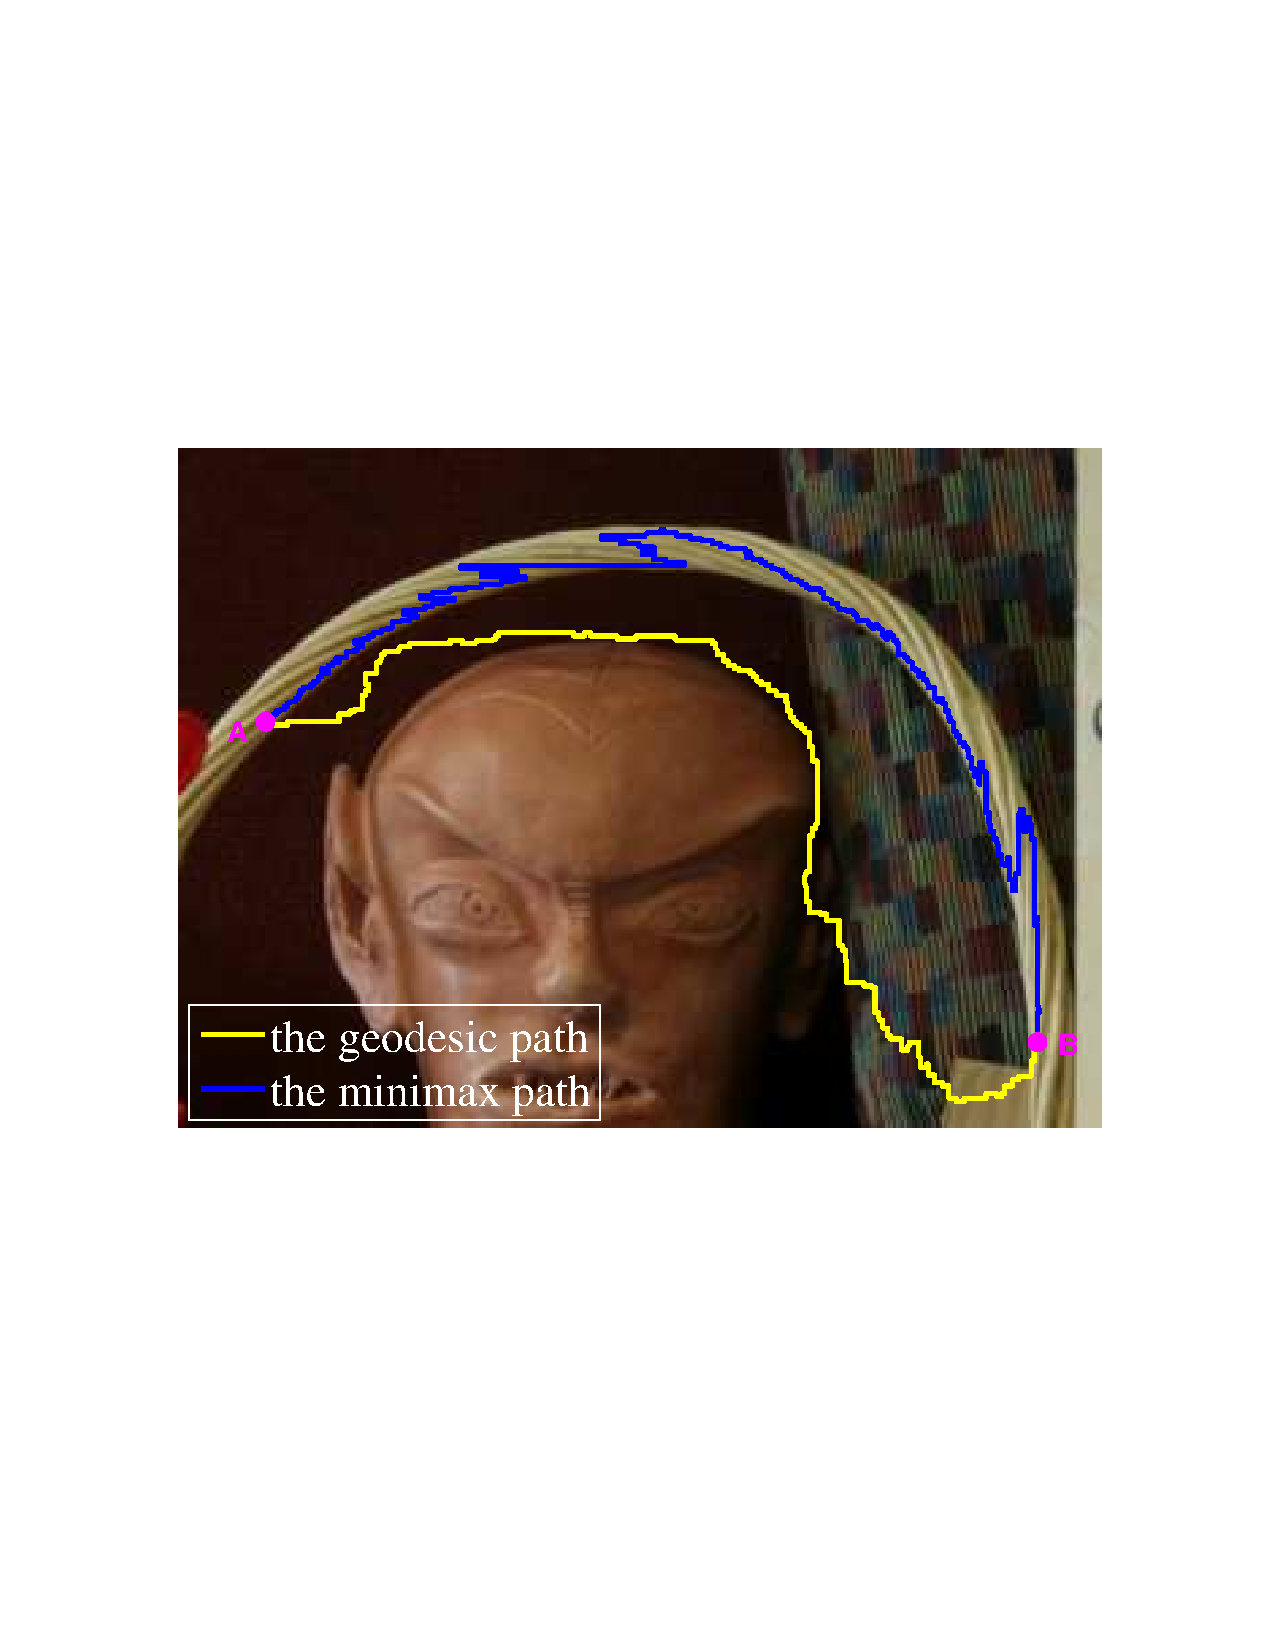
\includegraphics[width=0.8\linewidth]{path.pdf}
    \captionsetup{skip=1pt}
    \caption{}
    \label{fig:minimax_path:path}
\end{subfigure}
\hspace{0.3cm}
\begin{subfigure}[b]{0.18\linewidth}
    \centering
    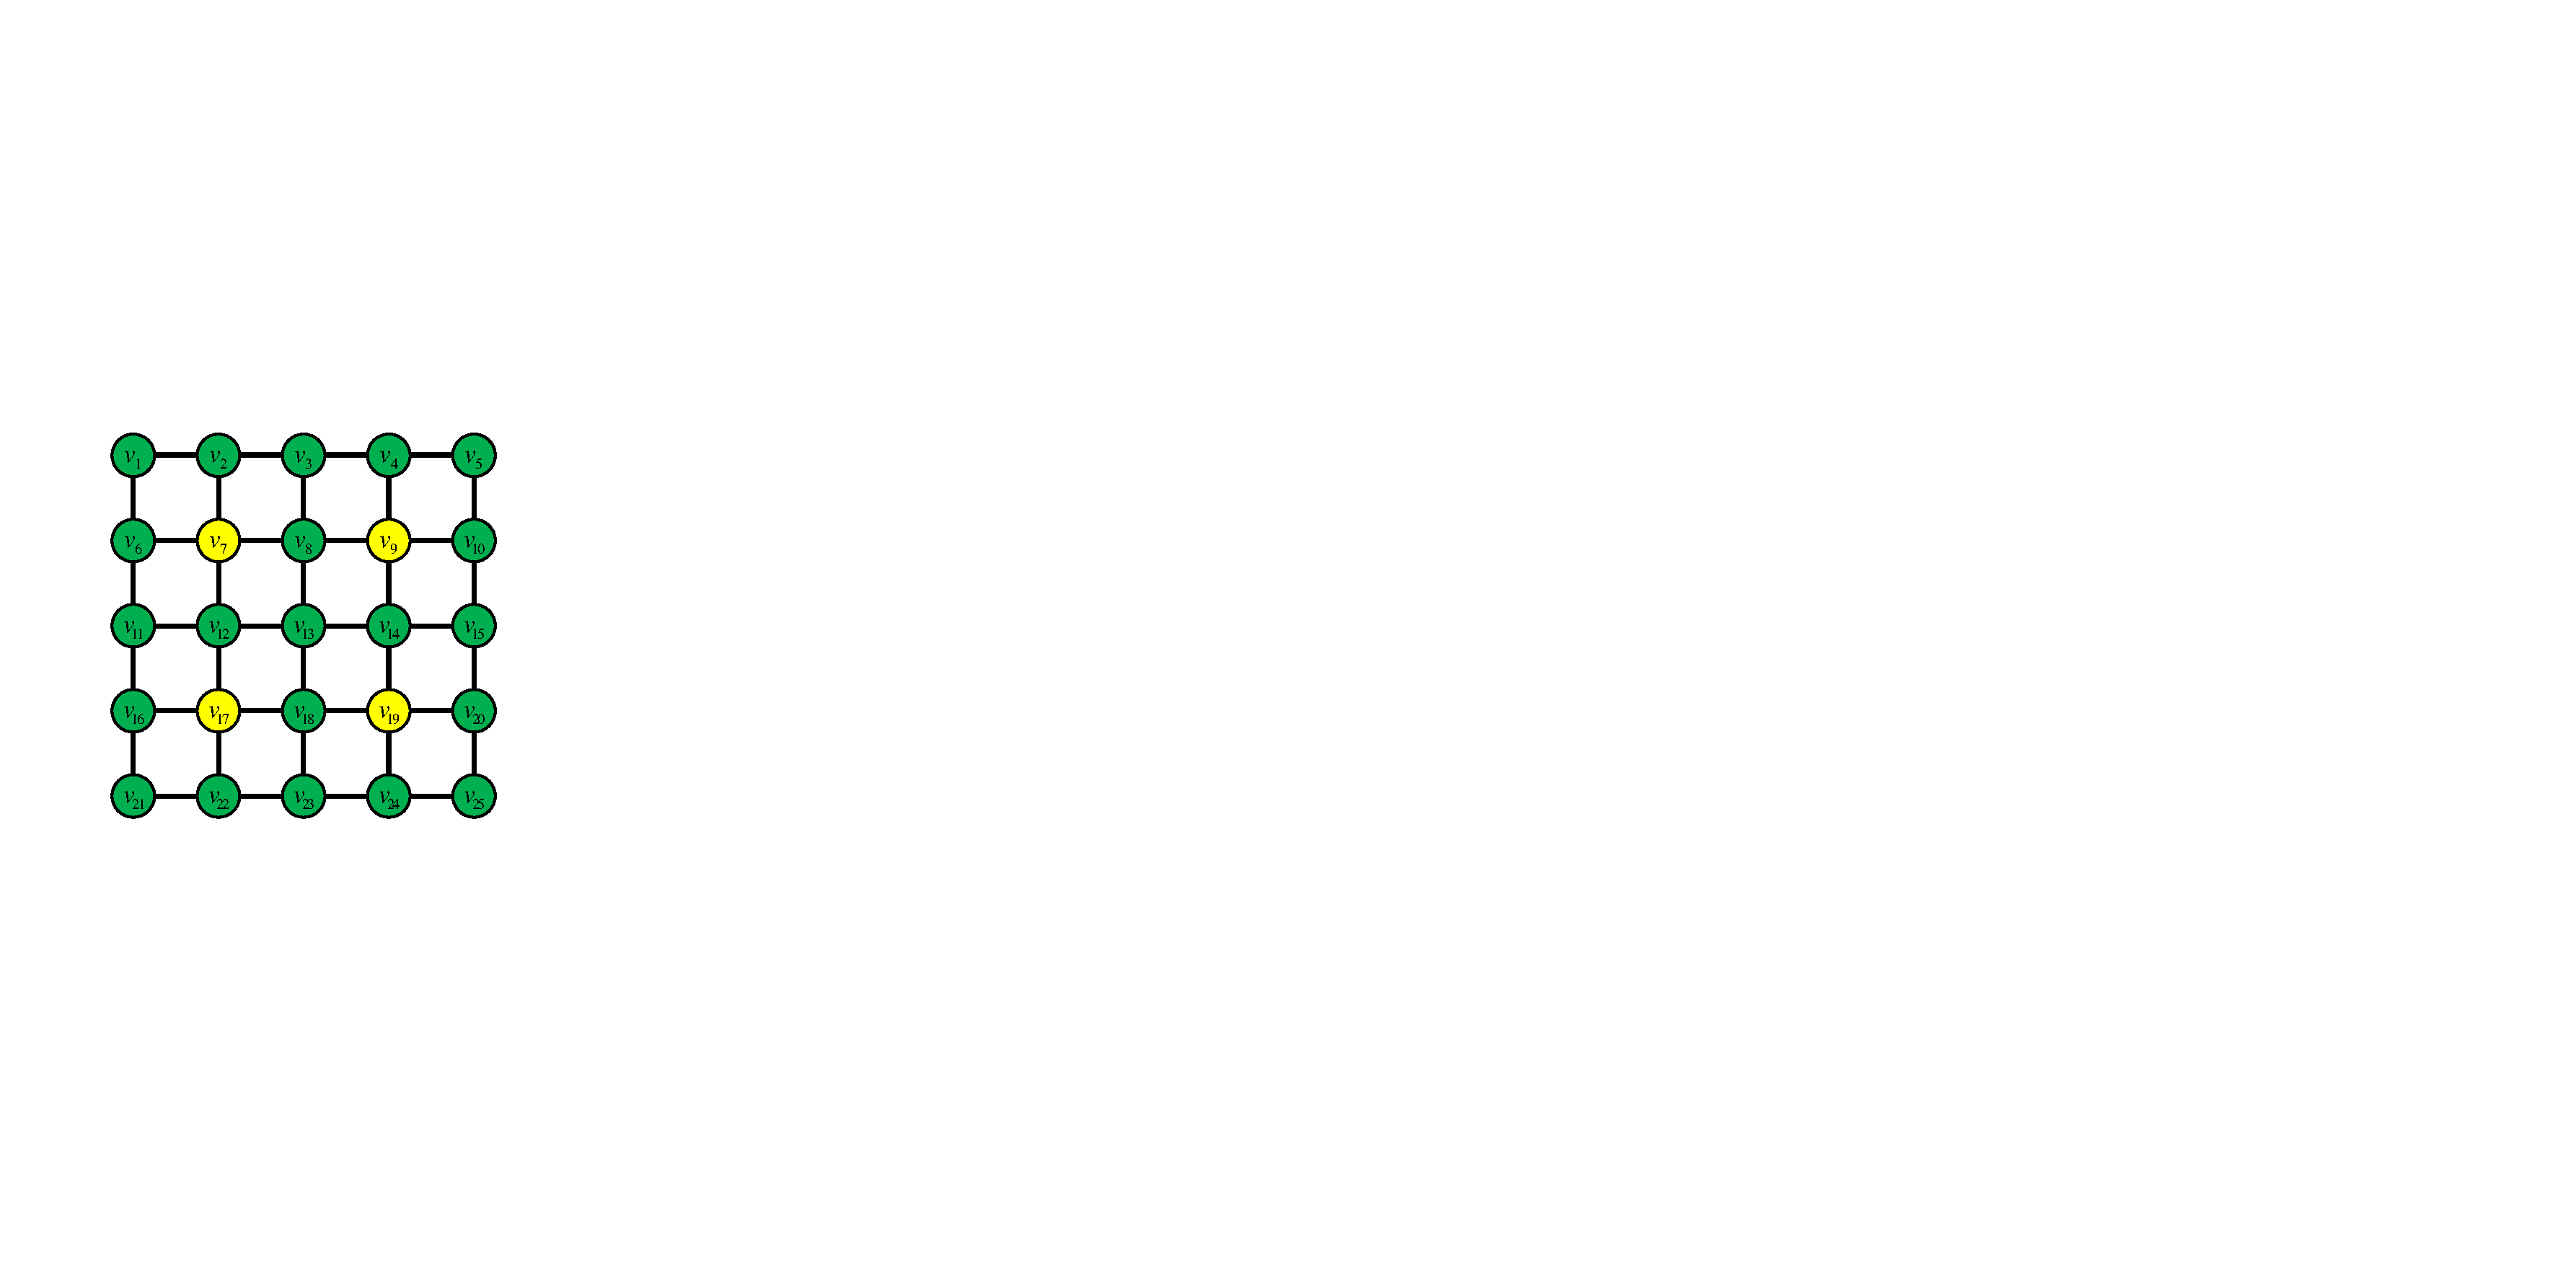
\includegraphics[width=0.6\linewidth]{interpolation_tree_1.pdf}
    \captionsetup{skip=1pt}
    \caption{}
    \label{fig:minimax_path:interpolation_tree_1}
\end{subfigure}
\begin{subfigure}[b]{0.18\linewidth}
    \centering
    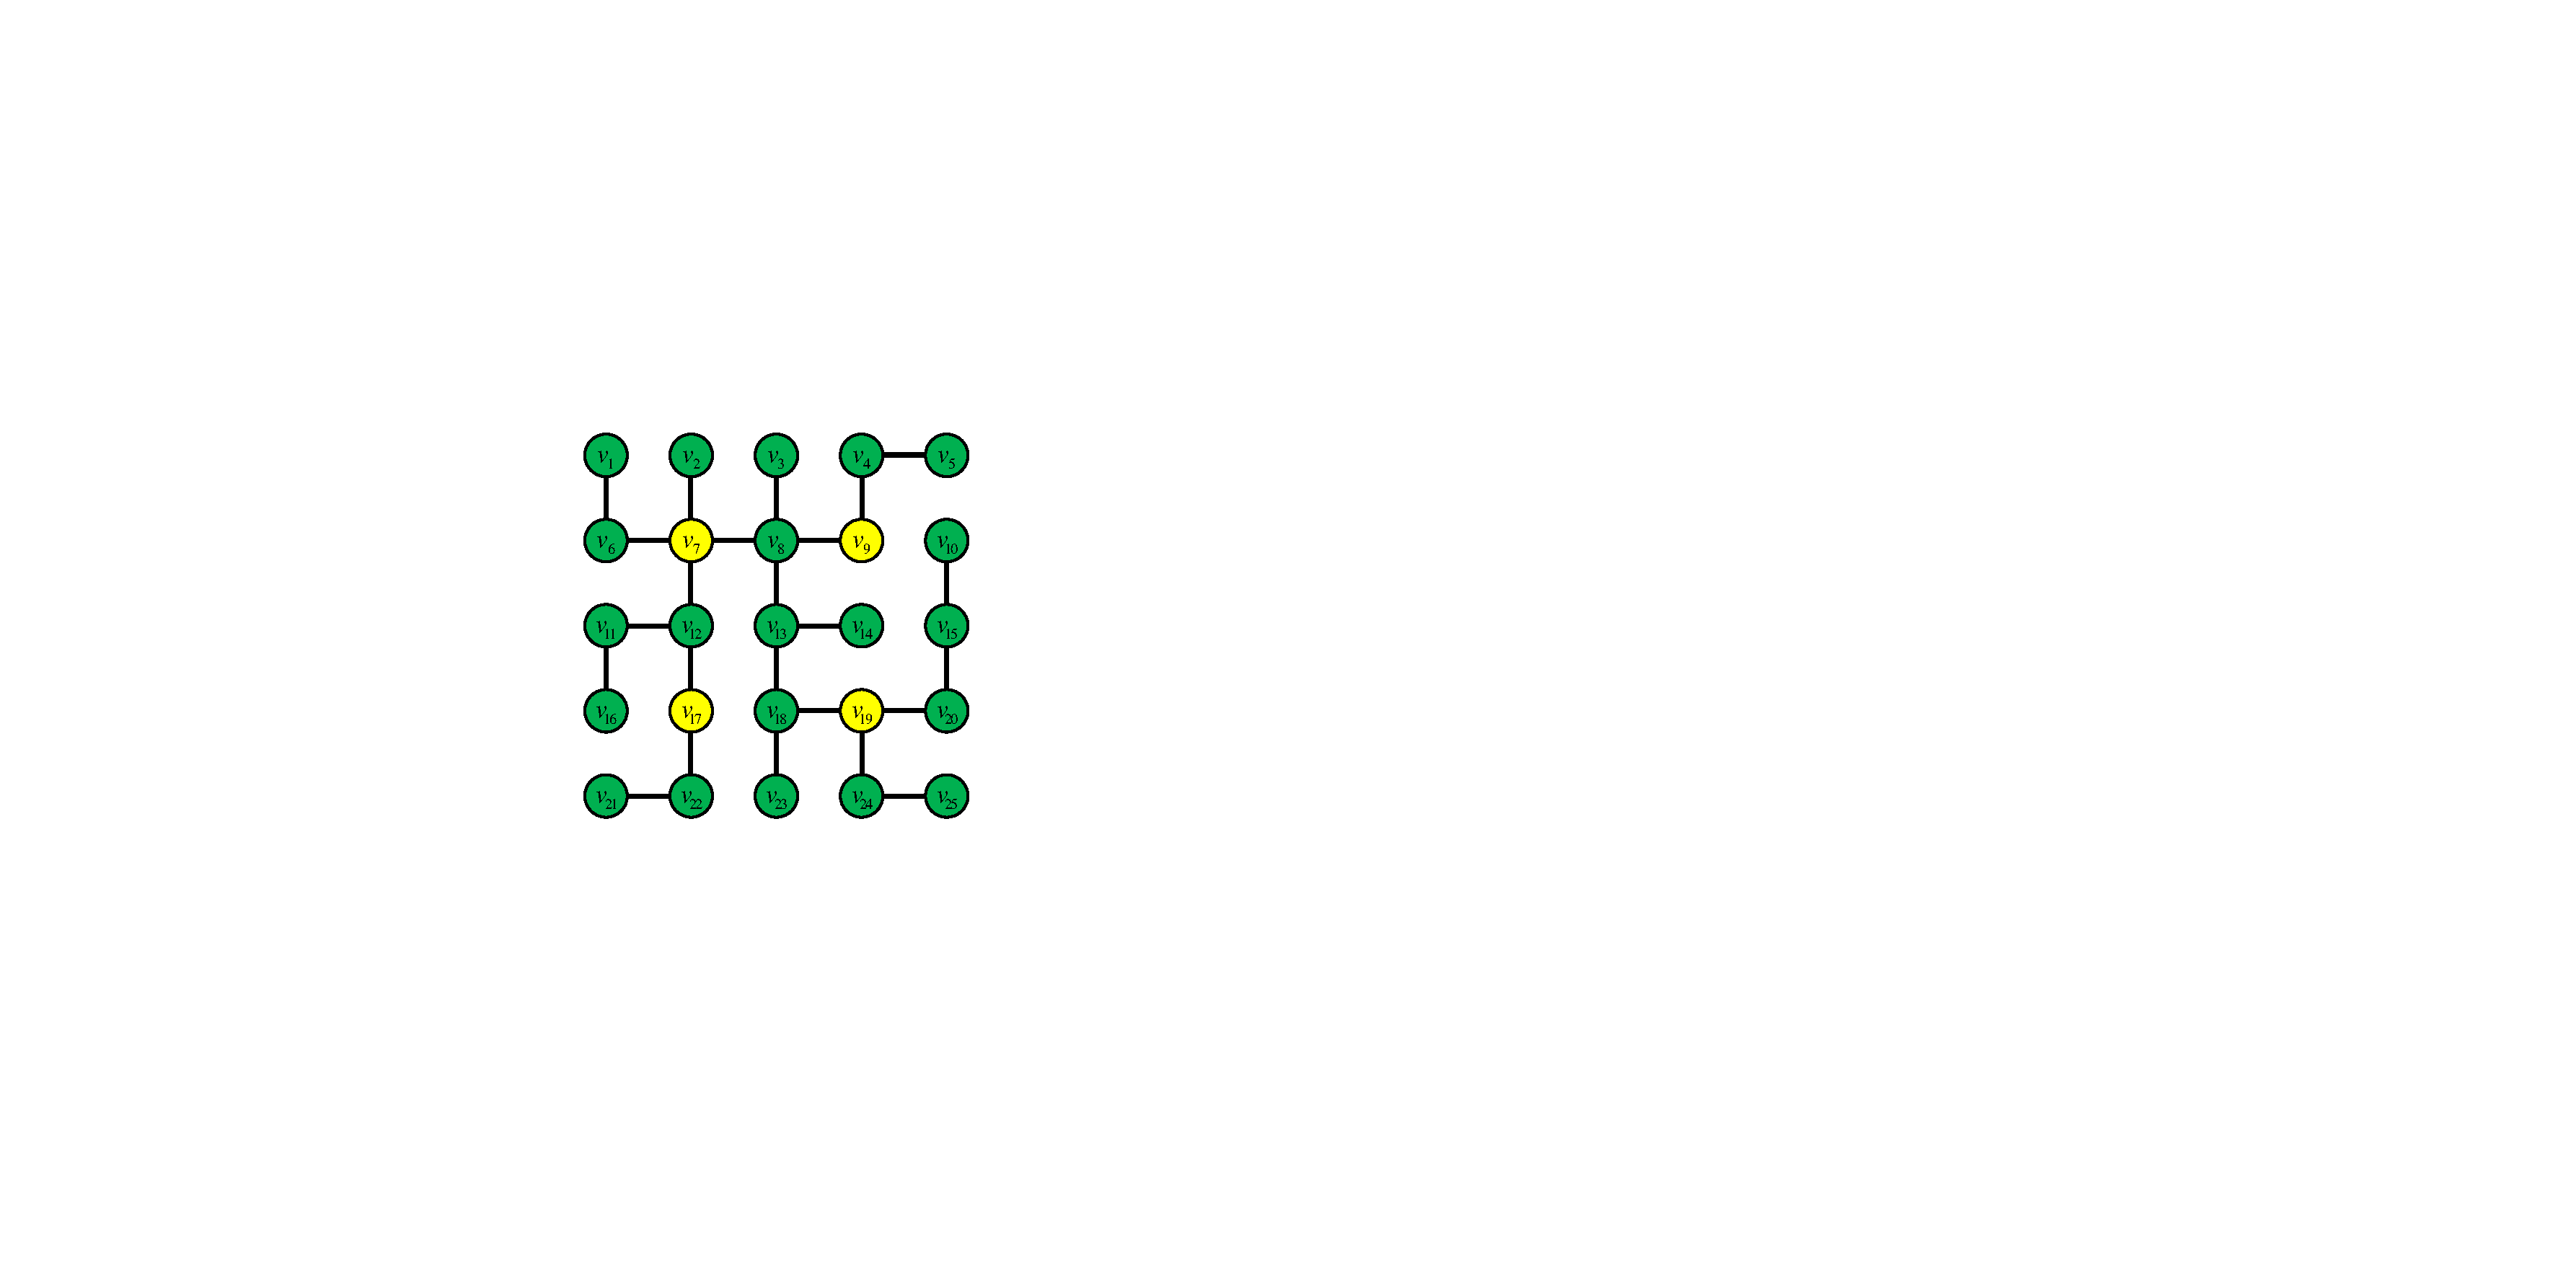
\includegraphics[width=0.6\linewidth]{interpolation_tree_2.pdf}
    \captionsetup{skip=1pt}
    \caption{}
    \label{fig:minimax_path:interpolation_tree_2}
\end{subfigure}
\begin{subfigure}[b]{0.18\linewidth}
    \centering
    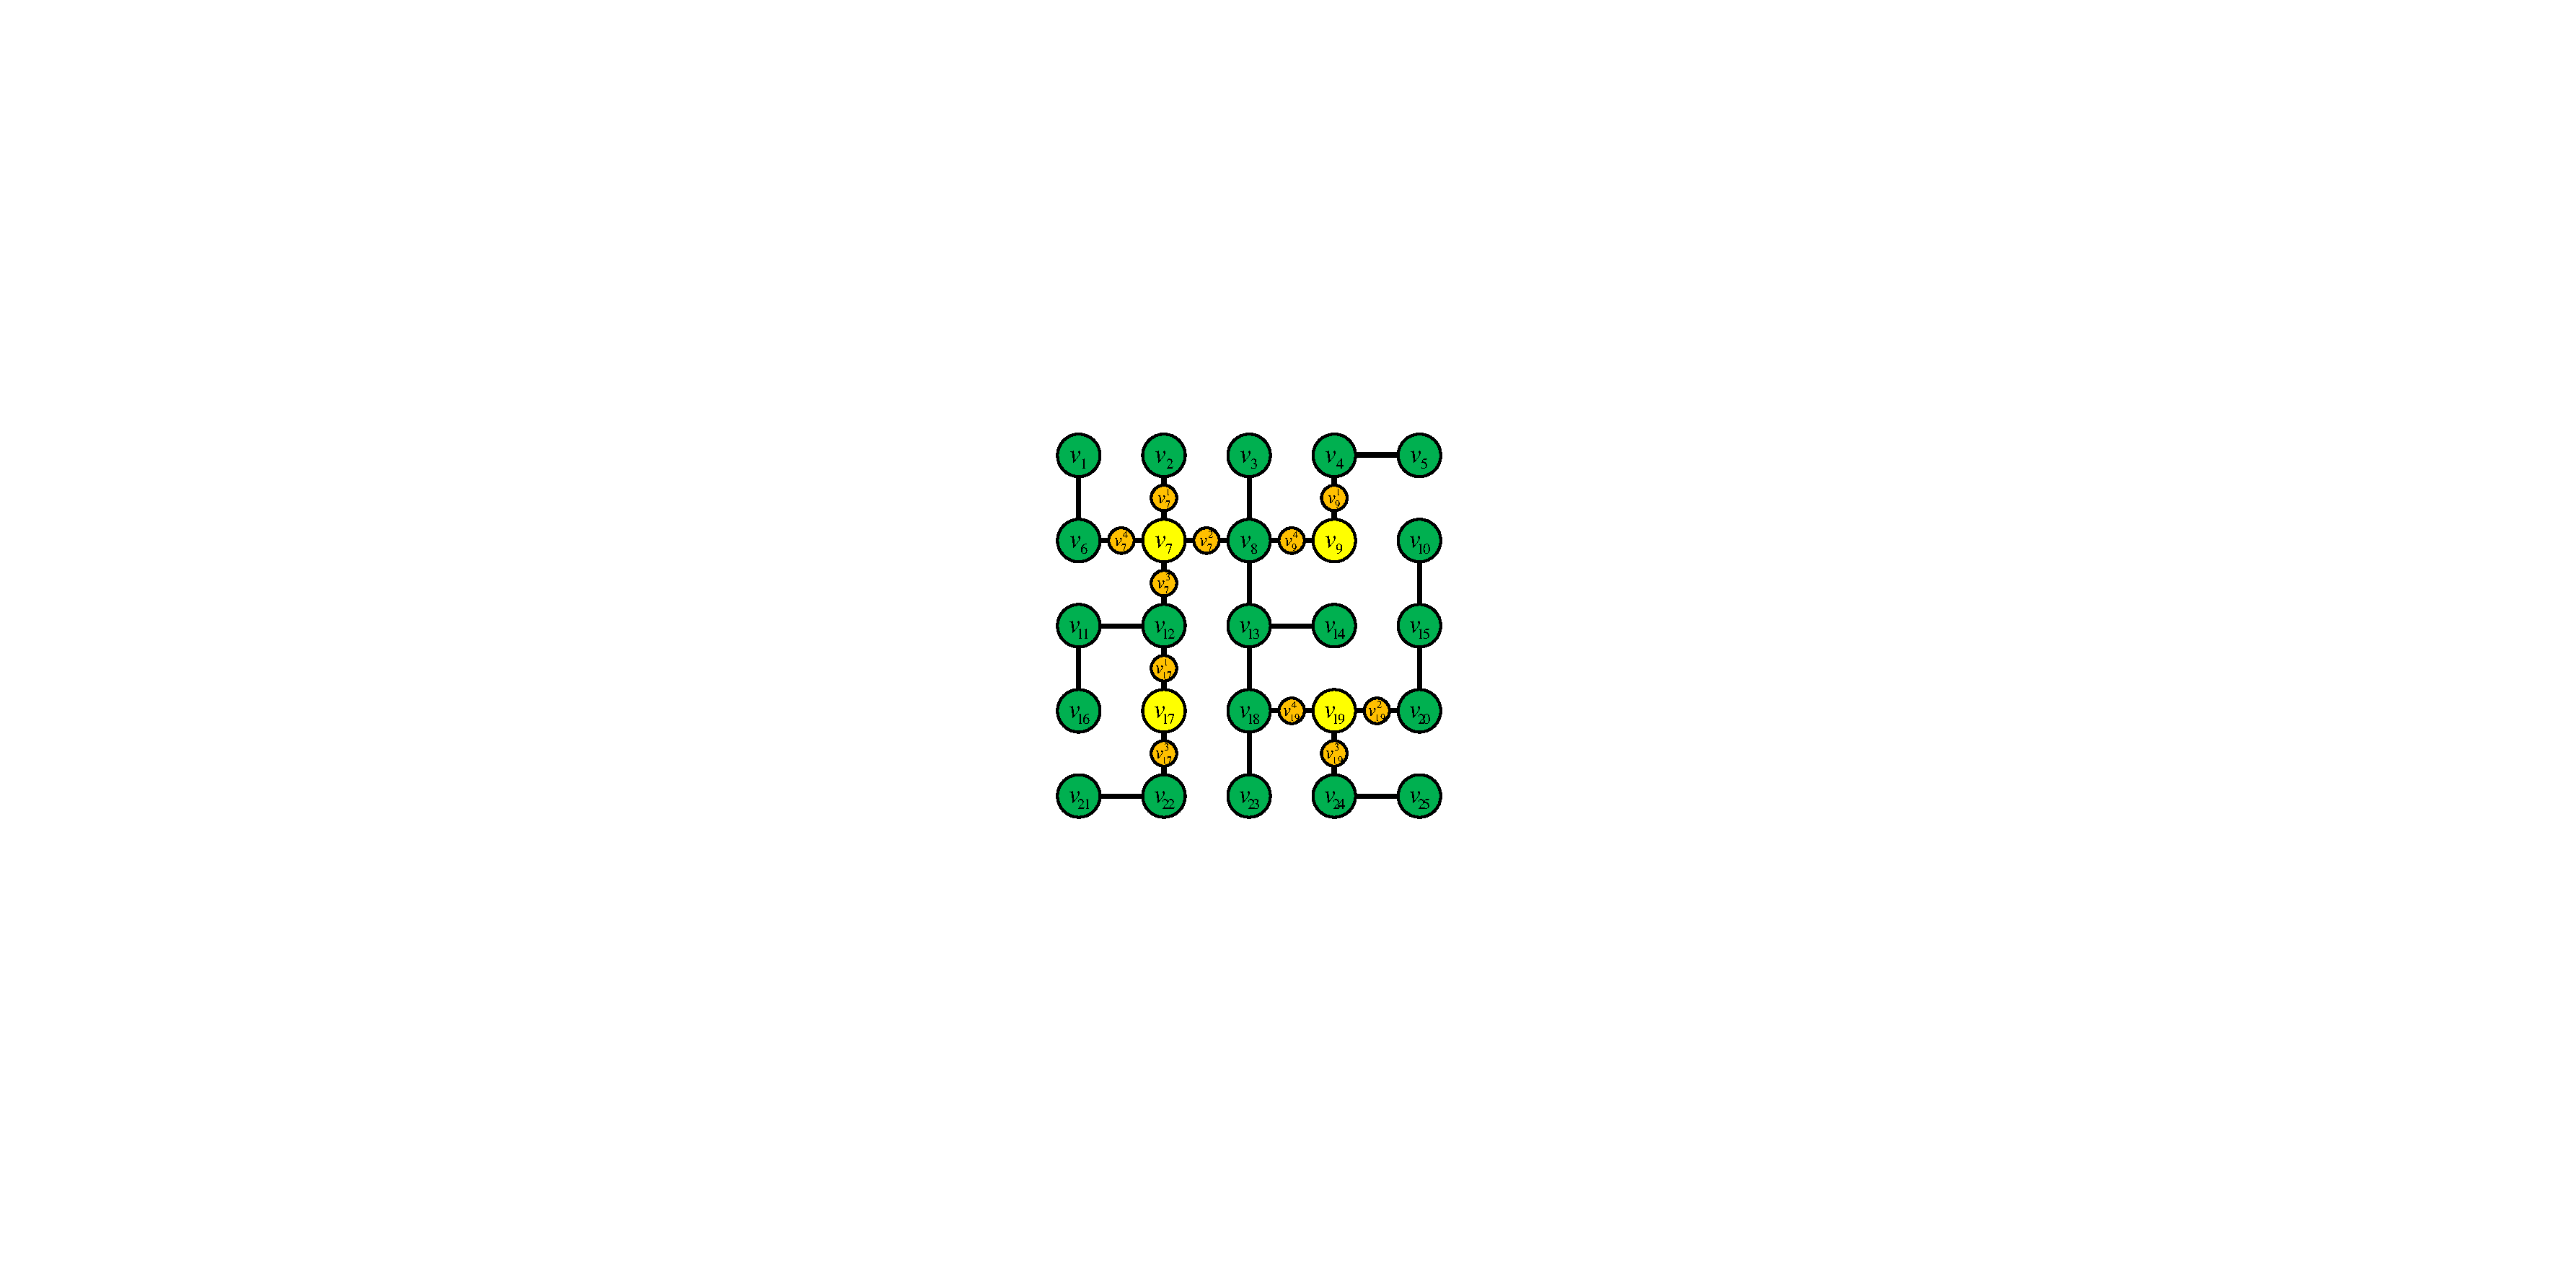
\includegraphics[width=0.6\linewidth]{interpolation_tree_3.pdf}
    \captionsetup{skip=1pt}
    \caption{}
    \label{fig:minimax_path:interpolation_tree_3}
\end{subfigure}
\begin{subfigure}[b]{0.18\linewidth}
    \centering
    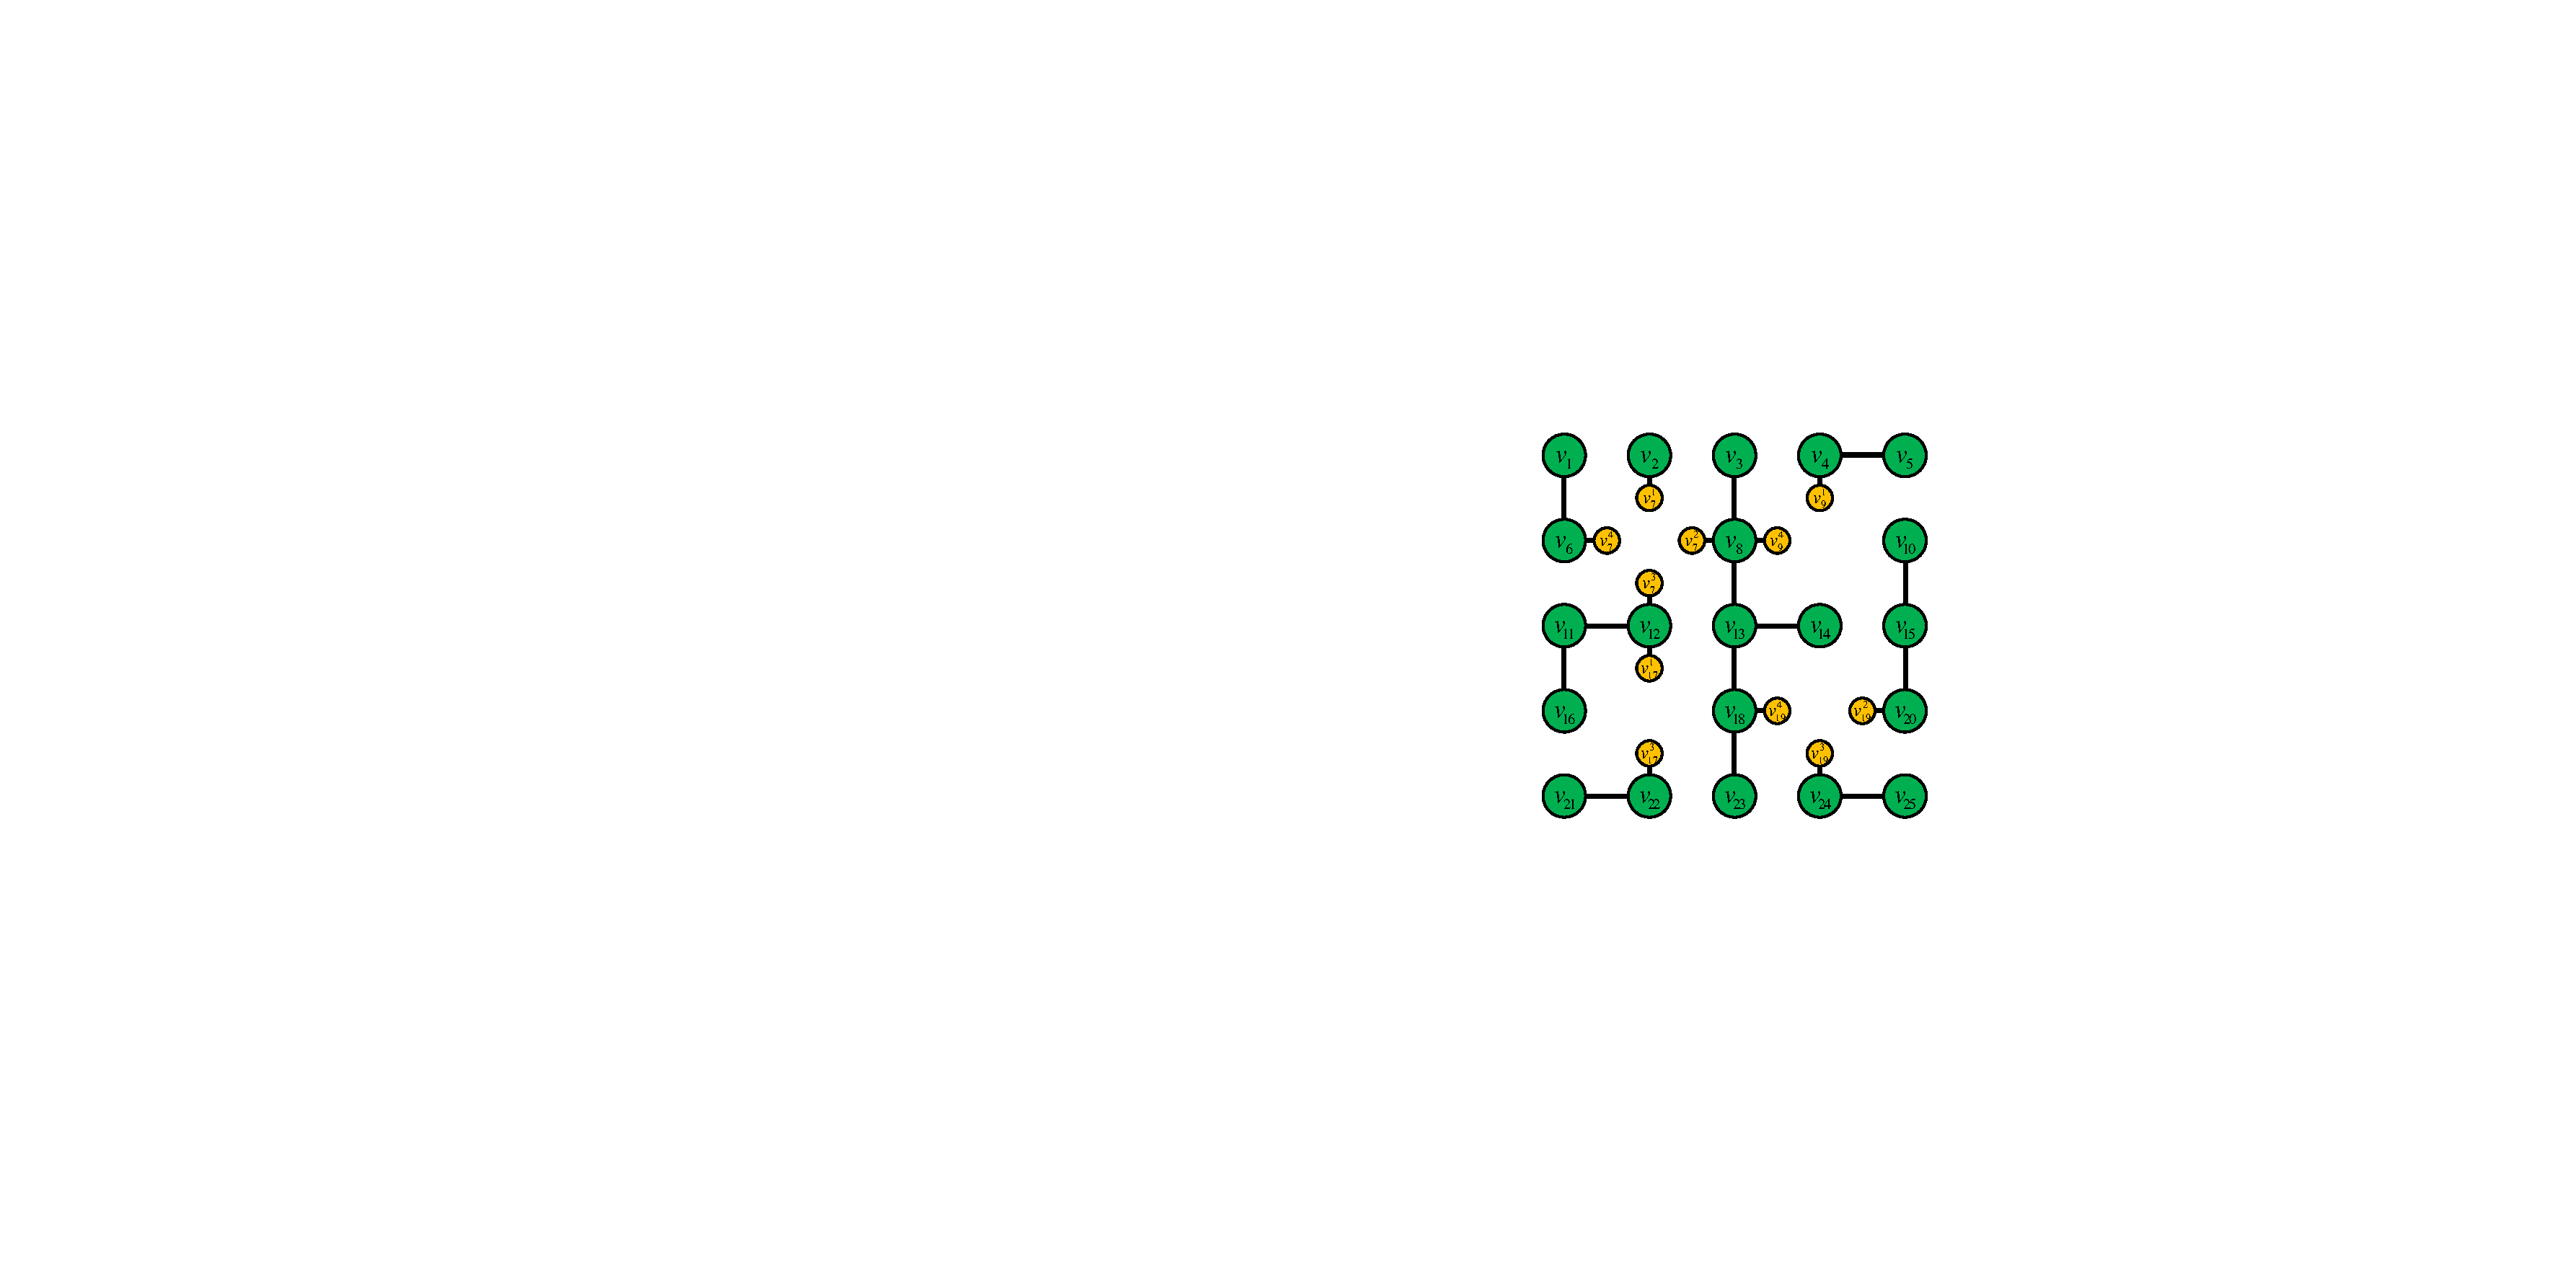
\includegraphics[width=0.6\linewidth]{interpolation_tree_4.pdf}
    \captionsetup{skip=1pt}
    \caption{}
    \label{fig:minimax_path:interpolation_tree_4}
\end{subfigure}
\caption{The comparison between minimax path and geodesic path, and the procedure demonstration of obtaining an interpolation tree. (a) shows that the geodesic chooses the crossing edges path which has a large jump at the color boundaries as the path is almost on the flatten area and the length on flatten area is nearly zero. In contrast, the minimax path is more sensitive to color edges and is able to follow the structure of guidance image. (b) the graph representation $G$ of guidance image, where the green nodes are target pixels and yellow nodes denote seeds. (c) a MST of $G$. (d) the obtained interpolation tree by inserting orange auxiliary nodes into the MST. (e) the auxiliary nodes divide the interpolation tree into several parts by removing seeds.}
\label{fig:minimax_path}
\vspace{-0.3cm}
\end{figure*}
%
Here we identify what the essential ingredients of the ideal joint interpolation method are by disclosing the shortcomings of local upsampling methods. Kopf \etal~\cite{Kopf2007} introduced the first weighted average based upsampling formula~\eqref{eq:joint_bilateral}.
%
\begin{equation}
D(p) = \frac{ \sum\nolimits_{q \in \Omega_p \bigcap S} {w^e_{p,q}D(q)} }{ {\sum\nolimits_{q \in \Omega_p \bigcap S} {w^e_{p,q}}}} \quad  p \in \Omega \setminus S
\label{eq:joint_bilateral}
\end{equation}
%
where $\Omega$ denotes the entire image domain, $S$ stands for the seeds and $w^e_{p,q} = \exp ( - \frac{{d^2_e}(p, I(p)),(q, I(q)) }{\sigma^2_e} ) $. However, the user-specified window $\Omega_p$ and the Euclidean distance $d_e$~\cite{Kopf2007} defined on the five-dimensional space-color volume~\cite{Adams2009} are suboptimal to take advantage of the geometric structure of guidance image $I$ because both $\Omega_p$ and $d_e$ are not adaptive to the underlying geometric structure of the guidance image $I$. Liu \etal~\cite{Liu2013} substituted the Euclidean distance $d_e$~\cite{Kopf2007} with the geodesic distance $d_g$~\cite{Liu2013} and replaced the user-specified window selecting method with the $K$ nearest seeds choosing strategy. The interpolation formula~\eqref{eq:joint_geodesic} is still  problematic.
%
\begin{equation}
D(p) = \frac{ \sum\nolimits_{q \in \mathcal{K}_p} {w^g_{p,q}D(q)} }{ {\sum\nolimits_{q \in \mathcal{K}_p} w^g_{p,q}}} \quad  p \in \Omega \setminus S   \label{eq:joint_geodesic}
\end{equation}
%
where $w^g_{p,q} = \exp( - \frac{{d^2_g}(\pi _{{p},{q}}^g)}{\sigma^2_g}  )$  and $\mathcal{K}_p$ denotes the $K$ nearest seeds of the target pixel $p$. Specifically,
Liu \etal employ an iterative algorithm with $O(Mn)$ complexity to calculate the geodesic distance, as the computational cost for extracting all-pairs geodesic paths is $\log(n^2 \log n)$~\cite{Kopf2007}. But accurate approximation demands $M$ iterations, which is still  inefficient. Additionally, it is reasonable to expect that the quality of  results will increase with the number $K$ of reliable seeds. Unfortunately, Liu's $O(Kn)$ algorithm depends on $K$ too.

Above all, we argue that an ideal joint interpolation should have following properties:

\begin{enumerate}

  \item An ideal interpolation method should utilize a reliable seed choosing strategy which can automatically catch all the reliable seeds for any distribution.

  \item An ideal interpolation method should employ a geometric-aware similarity metric, which is sensitive to the underlying geometric structure of guidance image, to weight the contributions from reliable seeds.

  \item The implementation of an ideal interpolation method should be high-efficiency, especially for real-time applications, thus an algorithm with $O(n)$ complexity should be given the primary consideration.

\end{enumerate}




\subsection{The geometric aware minimax distance}
%
Similar to the well-known geodesic distance, the minimax distance (\ie the length of the minimax path) is another kind of geometric-aware metric which can be used to measure the similarities between seeds and target pixels. The minimax path is defined on the graph representation $G(V, E)$ (Fig.~\ref{fig:minimax_path:interpolation_tree_1}) of the guidance image $I$, where each pixel of $I$ corresponds to a node $p \in V$ and the first order neighborhood $(v_1, v_2)$ of pixels $v_1$ and $v_2$ denotes an edge $e_{v_1, v_2} \in E$ with length $d(e_{v_1, v_2}) = {\left\| {I({v_1}) - I({v_2})} \right\|_1} $. Thus the minimax path $\pi^m_{p,q}$ that links pixels $p$ and $q$ is ${\pi^m_{{p},{q}}} \in \mathop {\arg \min }\nolimits_{\pi_{{p},{q}} \in {\Pi _{{p},{q}}}} ({d_\infty }(\pi^m_{{p},{q}}))$, where ${\Pi _{pq}}$ denotes all the possible paths which connect the initial node $v_{{a_0}}=p$ and the destination vertex $v_{{a_m}}=q$ such that $\{ {{e_{{v_{{a_0}}},{v_{{a_1}}}}},{e_{{v_{{a_1}}},{v_{{a_2}}}}}, \ldots ,{e_{{v_{{a_{m - 1}}}},{v_{{a_m}}}}}} \} \subseteq E$, for any path $\pi_{v_{{a_0}}, v_{{a_m}}}  = ({v_{{a_0}}},{v_{{a_1}}}, \ldots ,{v_{{a_m}}})$, $v_{{a_i}} \in V$. Moreover, ${d_\infty(\pi_{v_{{a_0}}, v_{{a_m}}}) } = \max\nolimits_{i \in \{0,\cdots,m-1\}} \{ d({e_{{v_a}_{_i},{v_a}_{_{i+1}}}})\}$. Using the same symbols, the minimax distance $d({\pi^m_{{a_0},{a_m}}})$ of ${\pi^m_{{a_0},{a_m}}}$ can be written as $d({\pi^m_{{a_0},{a_m}}}) = \sum\nolimits_{i=0}^{m-1} {d({e_{{v_a}_{_i},{v_a}_{_{i + 1}}}})}$.

The minimax path is more sensitive to color transition than geodesic. Specifically, the minimax path, according to the definition, minimizes the maximal length of edges of a path whereas geodesic prefers the shortest path which tolerates large color transition on the path, as shown in Fig.~\ref{fig:minimax_path:path}. More importantly, unlike the fastest extracting all-pairs geodesic paths algorithm with $O(n^2 \log n)$ complexity~\cite{Liu2013}, Hu~\cite{Hu1961} proves that all-pairs minimax paths (shown in Fig.~\ref{fig:minimax_path:interpolation_tree_2}) can be represented by a minimum spanning tree (MST) which has an efficient extracting algorithm with $O(\log n)$ complexity~\cite{Chong2001}.

\subsection{A reliable seed choosing strategy}
%
A MST of the graph representation $G(V, E)$ of a depth map connects all points on the graph $G$ and the path linking two nodes along the MST is the minimax path between them~\cite{Hu1961}. We find that the seeds on the graph $G(V, E)$ separate the graph into $L$ different subgraphs $\Omega_i, 1 \leq i \leq L$ along a MST of the graph and thus form the boundary $B_i$ of these subgraphs. In Fig.~\ref{fig:minimax_path}, the yellow points demonstrate the boundary seeds. We can observe that the path that links any two interior nodes of two different subgraphs along the MST must pass through at least one boundary node (or seed). For example, the path linking $v_6$ and $v_8$ passes through $v_7$. Then, for each target pixel in the subgraph $\Omega_i$, using the depths of the boundary points $B_i$ to interpolate the depths of the target pixels in the subgraph $\Omega_i$ is more reliable than using other seeds because boundary points are the closest seeds to the target pixels in the sense of minimax distance, in other words, the minimax path from a non-boundary seed to any target pixel in $\Omega_i$ must pass through a boundary seed of $B_i$. We call these boundary seeds $B_i$ as the reliable seeds of the target pixels in $\Omega_i$ and only use their depths to interpolate the target pixels in $\Omega_i$.

The reliable seed choosing strategy has three major advantages. First, it automatically catches all reliable seeds for any target pixel and thus our interpolation algorithm can employ all reliable depth information to interpolate the depth of each target pixel. Second, it is not sensitive to the seed distribution and can be used to various seed distributions other than the uniform distribution taken by upsampling. Last but not least, the strategy can be integrated into a linear time joint interpolation algorithm without extra cost.


\subsection{A linear complexity joint interpolation algorithm}
%
Our interpolation formula is expressed as \eqref{eq:joint_mst}, which both takes the minimax distance as the similarity metric and employs our reliable seed choosing strategy to choose the interpolating seeds for each target pixel.
%
\begin{equation}
D(p) = \frac{ \sum\nolimits_{q \in B_i} {w^m_{p,q}D(q)} }{ {\sum\nolimits_{q \in B_i} {w^m_{p,q}}}} \quad p \in \Omega_i \setminus S \label{eq:joint_mst}
\end{equation}
%
where $w^m_{p,q} = \exp( - \frac{{d}(\pi_{{p},{q}}^m)}{\sigma_m})$ and $1 \leq i \leq L$.

The formula can be computed in a linear complexity by transforming the MST into an interpolation tree and updating depths along the interpolation tree $T$. Let $N(s)$ denote the neighborhood nodes which are connected to the seed $s$ by the MST. For each edge $e_{s, p}, p \in N(s)$, we insert an intermediate point $s_p$ into the middle of $s$ and $p$, as shown in Fig.~\ref{fig:minimax_path:interpolation_tree_3}, and assign $d(e_{s, s_p}) = \infty, d(e_{s_p, p}) = d(e_{s, p})$. Here, all auxiliary points are denoted as $A$. We can observe from Fig.~\ref{fig:minimax_path:interpolation_tree_4} that the interpolation tree $T$ is divided into $L$ subtrees $T_i$ by removing all seeds, and the depths of auxiliary nodes $\widetilde{B}_i = A \bigcap T_i$ determine the depths of the target pixels in the $T_i$. Then \eqref{eq:joint_mst} can be rewritten as
%
\begin{equation}
D(p) = \frac{ \sum\nolimits_{q \in \widetilde{B}_i} {w^t_{p,q}D(q)} }{ {\sum\nolimits_{q \in \widetilde{B}_i} {w^t_{p,q}}}} \quad p \in T_i \setminus A, \ 1 \leq i \leq L \label{eq:joint_mst_re}
\end{equation}
%
where $w_{p,q} = \exp( - \frac{{d}(\pi^t_{{p},{q}})}{\sigma_m})$ and $\pi^t_{{p},{q}}$ is the path that connects $p$ to $q$ along the interpolation tree $T$.


In order to obtain the updating formulae with linear complexity, we put
$\widetilde C(q) = D(q)$, $\widetilde W(q) = 1$, for $q \in S$; $\widetilde C(q) = D(s)$, $\widetilde W(q) = 1$, for $q \in A$; $\widetilde C(q) = 0$, $\widetilde W(q) = 0$, for a target pixel $q$, then \eqref{eq:joint_mst_re} can be further transformed into following forms.
%
\begin{align}
&C(p) = \sum\nolimits_{q \in T} {w^t_{p,q} \widetilde C(q)} \ \ W(p) = \sum\nolimits_{q \in T} {w^t_{p,q} \widetilde W(q)} \label{eq:cost_coe} \\
&D(p) = C(p)/ W(p) \quad p \in T_i \setminus A, \ 1 \leq i \leq L \label{eq:depth}
\end{align}
%
In \eqref{eq:cost_coe}, we replace $\widetilde{B}_i$ with $T$. Although the values of $C(p)$ and $W(p)$ for $p \in  T_i \setminus A$ receive supports from all other nodes on the interpolation tree $T$ according to \eqref{eq:cost_coe}, the depths of target pixels in $T_i$ only depend on the depths of auxiliary nodes $\widetilde{B}_i$ as the length of edge between the seed and its auxiliary points is set as infinity.

Yang~\cite{Yang2012} shows that the non-local cost aggregation form defined on the tree as $C(p)$ and $W(p)$ can be efficiently figured out by traversing the tree structure of the interpolation tree $T$ in two sequential passes. Initially, we visit the nodes of $T_p$ using the breadth first traversal algorithm to assign each node $v_i$ an order $i$ based on the visit sequence with the property that if $v_i$ is the father of $v_j$, then $i \leqslant j$, where $ 1 \leqslant i,j \leqslant \#T_p$, $\#T_p$ denotes the nodes number of $T_p$. In the first pass, while the tree is traced from $v_{\#T_p}$ to $v_{1}$, ${C^ \uparrow }(v_i)$ and ${W^ \uparrow }(v_i)$ are not updated until all its children have been updated by the updating formulae~\eqref{eq:c_uparrow}~\eqref{eq:w_uparrow}.
%
\begin{align}
&{{C}^ \uparrow }(P(v_i)) = {{C}^ \uparrow }(P(v_i)) + {{w^t_{v_i,P(v_i)}}{{C}^ \uparrow }(v_i)} \label{eq:c_uparrow}\\
&{{W}^ \uparrow }(P(v_i)) = {{W}^ \uparrow }(P(v_i)) + {{w^t_{v_i,P(v_i)}}{{W}^ \uparrow }(v_i)} \label{eq:w_uparrow}
\end{align}
%
where ${C^ \uparrow }(v)$ and ${W^ \uparrow }(v)$ are initialized as $\widetilde{C}(v)$ and $\widetilde{W}(v)$, $P(v)$ records the father of node $v$, both ${C^ \uparrow }(v)$ and ${W^ \uparrow }(v)$ are the intermediate aggregated results. In the second pass, we employ the updating formulae~\eqref{eq:c}~\eqref{eq:w} to renew $C(v)$ and $W(v)$ when the tree is traversed from $v_1$ to $v_{\#T_p}$. At last, we use \eqref{eq:depth} to estimate final interpolation depths.
%
\begin{align}
& C(v_i) = {w^t_{P(v_i),v_i}}{\widetilde{C}({P(v_i)})} + (1 - {w^{t^2}_{v_i,P(v_i)}}){C^ \uparrow }(v_i) \label{eq:c}\\
& W(v_i) = {w^t_{P(v_i),v_i}}{\widetilde{W}({P(v_i)})} + (1 - {w^{t^2}_{v_i,P(v_i)}}){W^ \uparrow }(v_i) \label{eq:w}
\end{align}
%

The computational complexity of our method consists of two parts: the cost of extracting a MST from the graph representation $G$ of the guidance image $I$ and the cost of updating \eqref{eq:c_uparrow}~\eqref{eq:w_uparrow}~\eqref{eq:c}~\eqref{eq:w}. In \eqref{eq:c_uparrow}~\eqref{eq:w_uparrow}~\eqref{eq:c}~\eqref{eq:w}, ${w^t_{P(v_i),v_i}}$ only depends on the edge weights of the interpolation tree $T$ and can be pre-computed in linear complexity. Thus, only a total of 6 addition/subtraction operations and 7 multiplication/division operations are required for each node. So we can complete the interpolation task with $O(n)$ complexity disregarding the number $K$ of reliable seeds. The interpolation tree $T$ can be easily transformed from a MST with linear time by traversing the MST and inserting auxiliary nodes. To extract a MST, Karger~\etal~\cite{Karger1995} present a linear time randomized algorithm. Moreover, with a linear number of processors, the parallel algorithm~\cite{Chong2001} for the minimum spanning tree problem can solve the problem in $O(\log n)$ time. Above all, we conclude that the overall complexity of our algorithm is $O(n)$.


\begin{figure*}[t]
%\vspace{-0.5cm}
\begin{center}
\begin{subfigure}[b]{0.136\linewidth}
    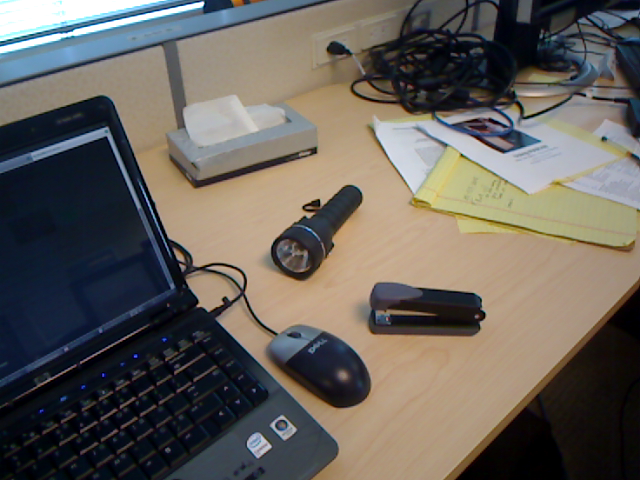
\includegraphics[width=\linewidth,height=1.3cm]{desk_structure_missing_color.png}
    %\captionsetup{skip=5pt}
    \label{fig:}
\end{subfigure}
\begin{subfigure}[b]{0.136\linewidth}
    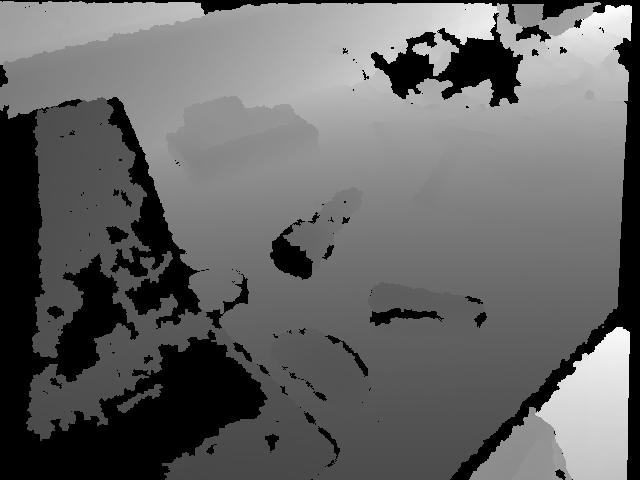
\includegraphics[width=\linewidth,height=1.3cm]{desk_structure_missing_depth.png}
    \label{fig:} %% label for first subfigure
\end{subfigure}
\begin{subfigure}[b]{0.136\linewidth}
    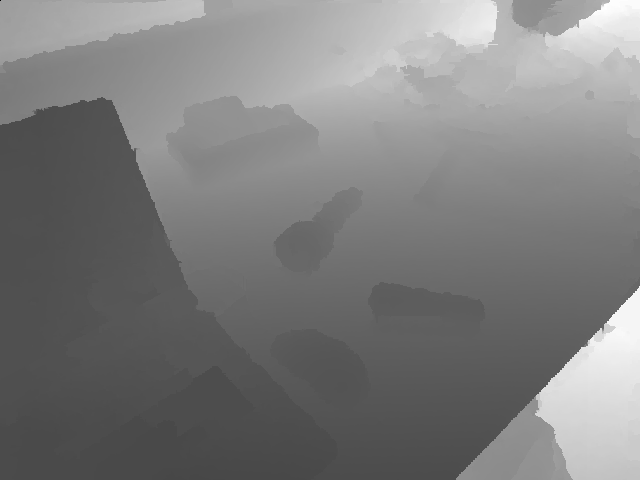
\includegraphics[width=\linewidth,height=1.3cm]{desk_structure_missing_inpainting.png}
    %\captionsetup{skip=5pt}
    \label{fig:}
\end{subfigure}
\begin{subfigure}[b]{0.136\linewidth}
    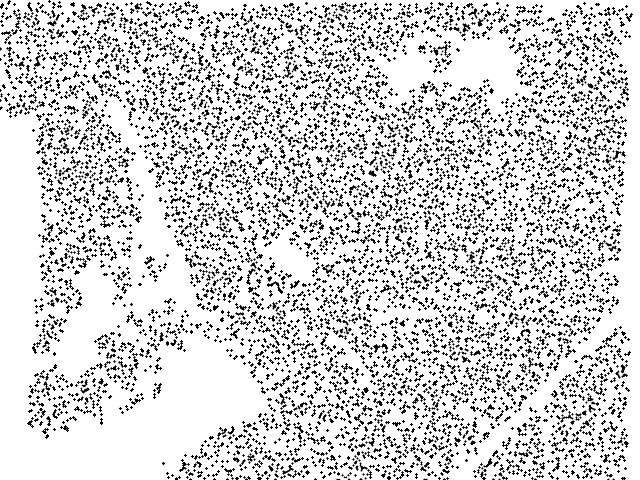
\includegraphics[width=\linewidth,height=1.3cm]{desk_random_missing_depth.png}
    \label{fig:} %% label for first subfigure
\end{subfigure}
\begin{subfigure}[b]{0.136\linewidth}
    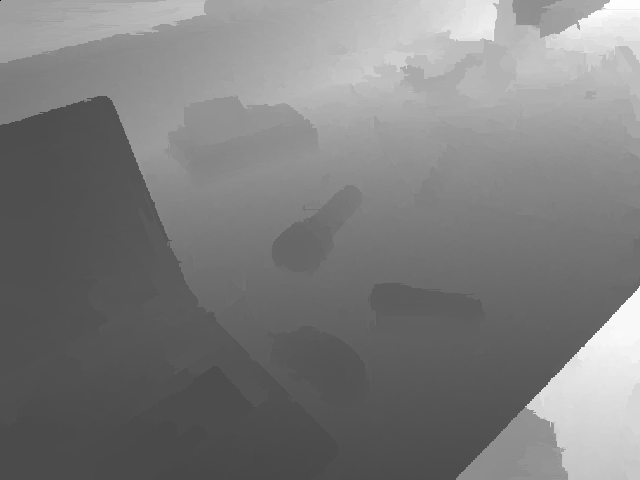
\includegraphics[width=\linewidth,height=1.3cm]{desk_random_missing_inpainting.png}
    %\captionsetup{skip=5pt}
    \label{fig:}
\end{subfigure}
\begin{subfigure}[b]{0.136\linewidth}
    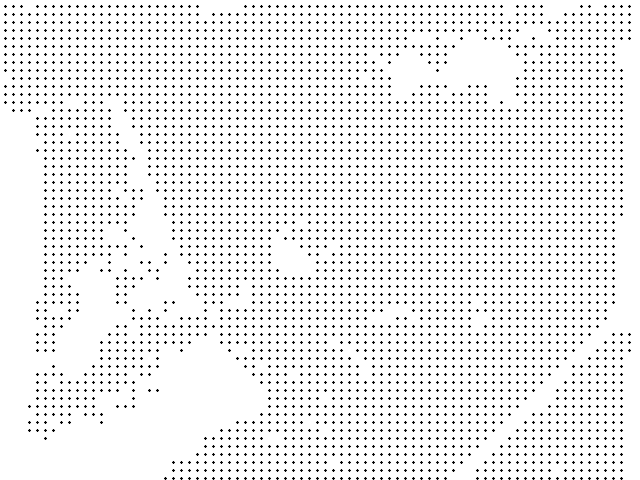
\includegraphics[width=\linewidth,height=1.3cm]{desk_upsampling_depth.png}
    \label{fig:} %% label for first subfigure
\end{subfigure}
\begin{subfigure}[b]{0.136\linewidth}
    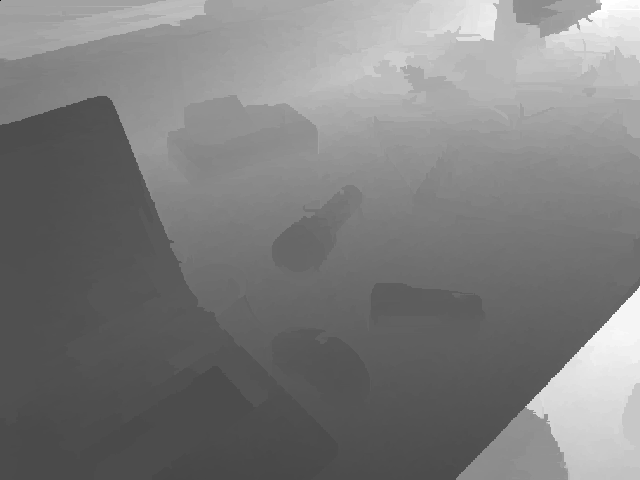
\includegraphics[width=\linewidth,height=1.3cm]{desk_upsampling_inpainting.png}
    \label{fig:} %% label for first subfigure
\end{subfigure}

%%%%%%%%%%%%%%%%%%%%%%%%%%%%%%%%%%%%%%%%%%%%%%%%%%%%%%%%%%%%%%%%%%
\vspace{-0.4cm}
\begin{subfigure}[b]{0.136\linewidth}
    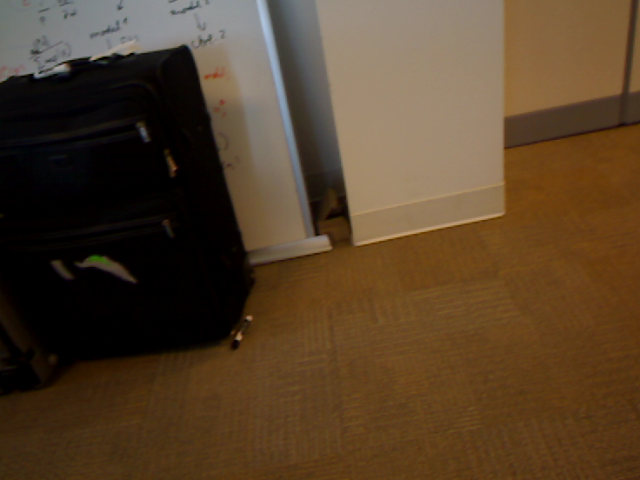
\includegraphics[width=\linewidth,height=1.3cm]{case_structure_missing_color.png}
    \captionsetup{skip=2pt}
    \caption{}
    \label{fig:structure_missing_color}
\end{subfigure}
\begin{subfigure}[b]{0.136\linewidth}
    
\includegraphics[width=\linewidth,height=1.3cm]{case_structure_missing_depth.png}
    \captionsetup{skip=2pt}
    \caption{}
    \label{fig:structure_missing_depth}
\end{subfigure}
\begin{subfigure}[b]{0.136\linewidth}
    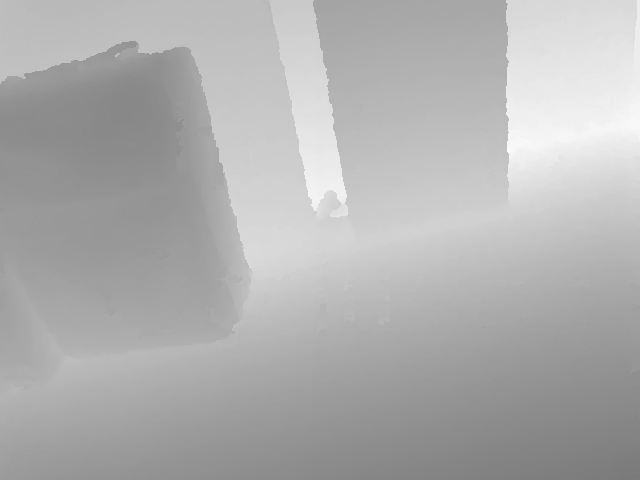
\includegraphics[width=\linewidth,height=1.3cm]{case_structure_missing_inpainting.png}
    \captionsetup{skip=2pt}
    \caption{}
    \label{fig:structure_missing_inpainting}
\end{subfigure}
\begin{subfigure}[b]{0.136\linewidth}
    
\includegraphics[width=\linewidth,height=1.3cm]{case_random_missing_depth.png}
    \captionsetup{skip=2pt}
    \caption{}
    \label{fig:random_missing_depth}
\end{subfigure}
\begin{subfigure}[b]{0.136\linewidth}
    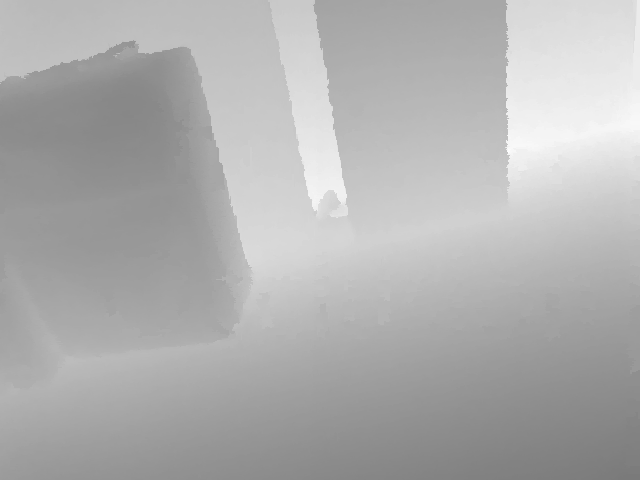
\includegraphics[width=\linewidth,height=1.3cm]{case_random_missing_inpainting_new.png}
    \captionsetup{skip=2pt}
    \caption{}
    \label{fig:random_missing_inpainting}
\end{subfigure}
\begin{subfigure}[b]{0.136\linewidth}
    
\includegraphics[width=\linewidth,height=1.3cm]{case_upsampling_depth.png}
    %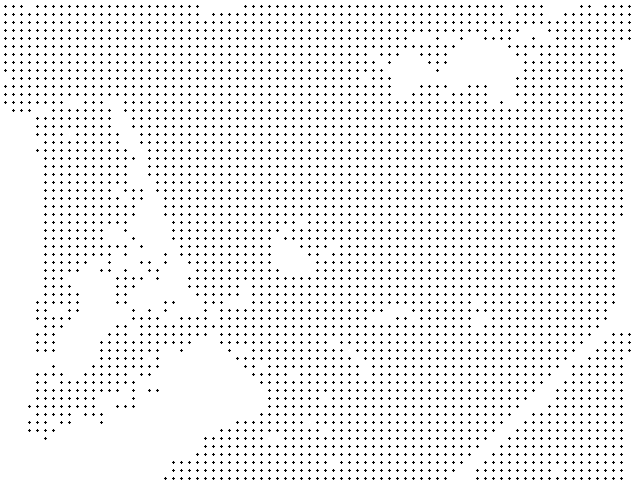
\includegraphics[width=\linewidth]{t.png}
    \captionsetup{skip=2pt}
    \caption{}
    \label{fig:upsampling_depth}
\end{subfigure}
\begin{subfigure}[b]{0.136\linewidth}
    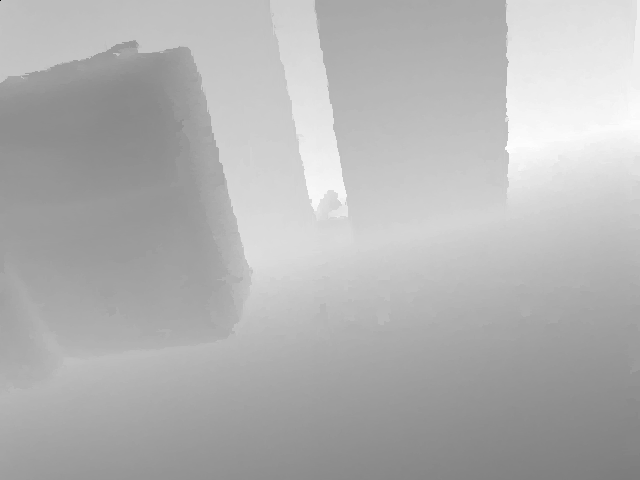
\includegraphics[width=\linewidth,height=1.3cm]{case_upsampling_inpainting_new.png}
    \captionsetup{skip=2pt}
    \caption{}
    \label{fig:upsampling_inpainting}
\end{subfigure}
\end{center}
%\vspace{-0.6cm}
\caption{ Visual illustration of the interpolation results for real word data. (a) the registered guidance images. (b) the depth maps which are used as seed for structure missing. (c) the restoration results for structure missing. (d) the seed distribution for simultaneous $5\%$ random missing and structure missing. (e) the inpainted results of (d). (f) the seed distribution for simultaneous 8X upsampling and structure missing. (g) the upsampled results of (f).}
\label{fig:visual_illustration}
\vspace{-0.2cm}
\end{figure*}


\begin{table}[!t]\fontsize{7pt}{0.4\baselineskip}\selectfont
%\vspace{-0.5cm}
\caption{ We compare the proposed algorithm with state-of-the-art methods on the Middlebury dataset using percentage of bad matching pixels~\cite{Scharstein2002}, where the disparity error tolerance is $1$. DISC denotes the percentage of bad matching pixels at discontinuous regions and CONT stands for the percentage of bad matching pixels at continuous areas.}
\centering
%\begin{tabularx}{\textwidth}{@{}|l|l|YYYY|YYYY|YYYY|@{}}
\begin{tabularx}{\textwidth}{@{}|l|l|llll|llll|@{}}
%\hline
\cline{1-10}
\multicolumn{2}{|c|}{  } & \multicolumn{4}{c|}{ Art} & \multicolumn{4}{c|}{ Book} \\
\cline{3-10}
\multicolumn{2}{|c|}{  } & 2X & 4X & 8X & 16X  & 2X & 4X & 8X & 16X  \\
\cline{1-10}
\multirow{2}{*}{AR}
                            & DISC
                            & 0.15 & 0.24 & 0.32 & 0.41
                            & 0.12 & 0.23 & 0.34 & 0.39 \\
                            & CONT
                            & 0.03 & 0.06 & 0.10 & 0.17
                            & 0.03 & 0.05 & 0.10 & 0.19 \\
\cline{1-10}
\multirow{2}{*}{ATGV}
                            & DISC
                            & 0.13 & 0.20 & 0.28 & 0.36
                            & 0.10 & 0.22 & 0.30 & 0.33 \\
                            & CONT
                            & 0.01 & 0.04 & 0.10 & 0.15
                            & 0.01 & 0.03 & 0.09 & 0.17 \\
\cline{1-10}
\multirow{2}{*}{NLA}
                            & DISC
                            & 0.17 & 0.27 & 0.39 & 0.48
                            & 0.22 & 0.33 & 0.41 & 0.49 \\
                            & CONT
                            & 0.01 & 0.04 & 0.07 & 0.12
                            & 0.02 & 0.04 & 0.08 & 0.18 \\
\cline{1-10}
\multirow{2}{*}{JBL}
                            & DISC
                            & 0.16 & 0.24 & 0.39 & 0.49
                            & 0.19 & 0.27 & 0.41 & 0.49 \\
                            & CONT
                            & 0.01 & 0.03 & 0.06 & 0.12
                            & 0.01 & 0.02 & 0.05 & 0.16 \\
\cline{1-10}
\multirow{2}{*}{JG}
                            & DISC
                            & 0.11 & 0.19 & 0.30 & 0.36
                            & 0.06 & 0.18 & 0.18 & 0.43 \\
                            & CONT
                            & 0.03 & 0.05 & 0.08 & 0.12
                            & 0.03 & 0.05 & 0.09 & 0.17 \\
\cline{1-10}
\multirow{2}{*}{Ours }
                            & DISC
                            & 0.04 & 0.09 & 0.16 & 0.22
                            & 0.02 & 0.06 & 0.09 & 0.15 \\
                            & CONT
                            & 0.01 & 0.03 & 0.07 & 0.12
                            & 0.01 & 0.04 & 0.08 & 0.13 \\
\cline{1-10}
\end{tabularx}
\label{tab:PBP}
%\vspace{-0.2cm}
\end{table}



%-------------------------------------------------------------------------
\section{Experiments}
\label{sec:experiments}


We implement our algorithm using Matlab on a Desktop computer with 4 GB memory. Parameter sensitivity and computation analysis are offered. We also exhibit the quantitative and visual evaluation of interpolation results.

\subsection{Quantitative and Visual Evaluation}



We compare our method with five methods which are JBL~\cite{Kopf2007}, JG~\cite{Liu2013}, ATGV~\cite{Ferstl_ICCV_2013}, NLA~\cite{Yang2012} and AR~\cite{YangJingyu2012} respectively. For fair comparison, we subscribe the 2X, 4X, 8X, 16X upsampling results of Art and Book of the Middlebury Stereo Datasets from original authors. In the experiments, the low resolution depth images are obtained by downsampling and we use the percentage of bad matching pixels (PBP)~\cite{Scharstein2002} to evaluate the performance at discontinuity regions and continuous areas, where the discontinuity regions are obtained by dilating 1-pixel wide edge of ground truth and the rest of image domain $\Omega$ are considered as continuous areas. In the experiments, we assign $\sigma_m = 0.05$ consistently.


The quantitative DISC (\ie the PBP at discontinuous regions) and CONT (\ie the PBP at continuous areas) evaluations are listed in Table~\ref{tab:PBP}. We find that the CONT of different methods are almost same, and the DISC indices, which reflect the edge preserving ability, distinguish different methods. Benefitting from the geometric-aware minimax path, our method achieves the lowest DISC ranks among all the methods as we expected.

We also use our method to process the depth map of Microsoft Kinect. We input the registered guidance images in Fig.~\ref{fig:structure_missing_color} and the deteriorated depth maps in Fig.~\ref{fig:structure_missing_depth}. The restoration results are illustrated in Fig.~\ref{fig:structure_missing_inpainting}.  We also exhibit the results of $5\%$ random missing inpainting and 8X upsampling in Fig.~\ref{fig:random_missing_inpainting},~\ref{fig:upsampling_inpainting} respectively. The seed distributions of both kinds of deterioration, which suffer from structure missing as Fig.~\ref{fig:structure_missing_depth} does, are shown in Fig.~\ref{fig:random_missing_depth},~\ref{fig:upsampling_depth} respectively. From Fig.~\ref{fig:visual_illustration}, we conclude that our method can produce satisfactory results for real world data and can be used in the working environment.

\begin{figure}[t]
%\vspace{-0.5cm}
\centering
\begin{subfigure}[b]{0.4\linewidth}
     %% label for first subfigure
    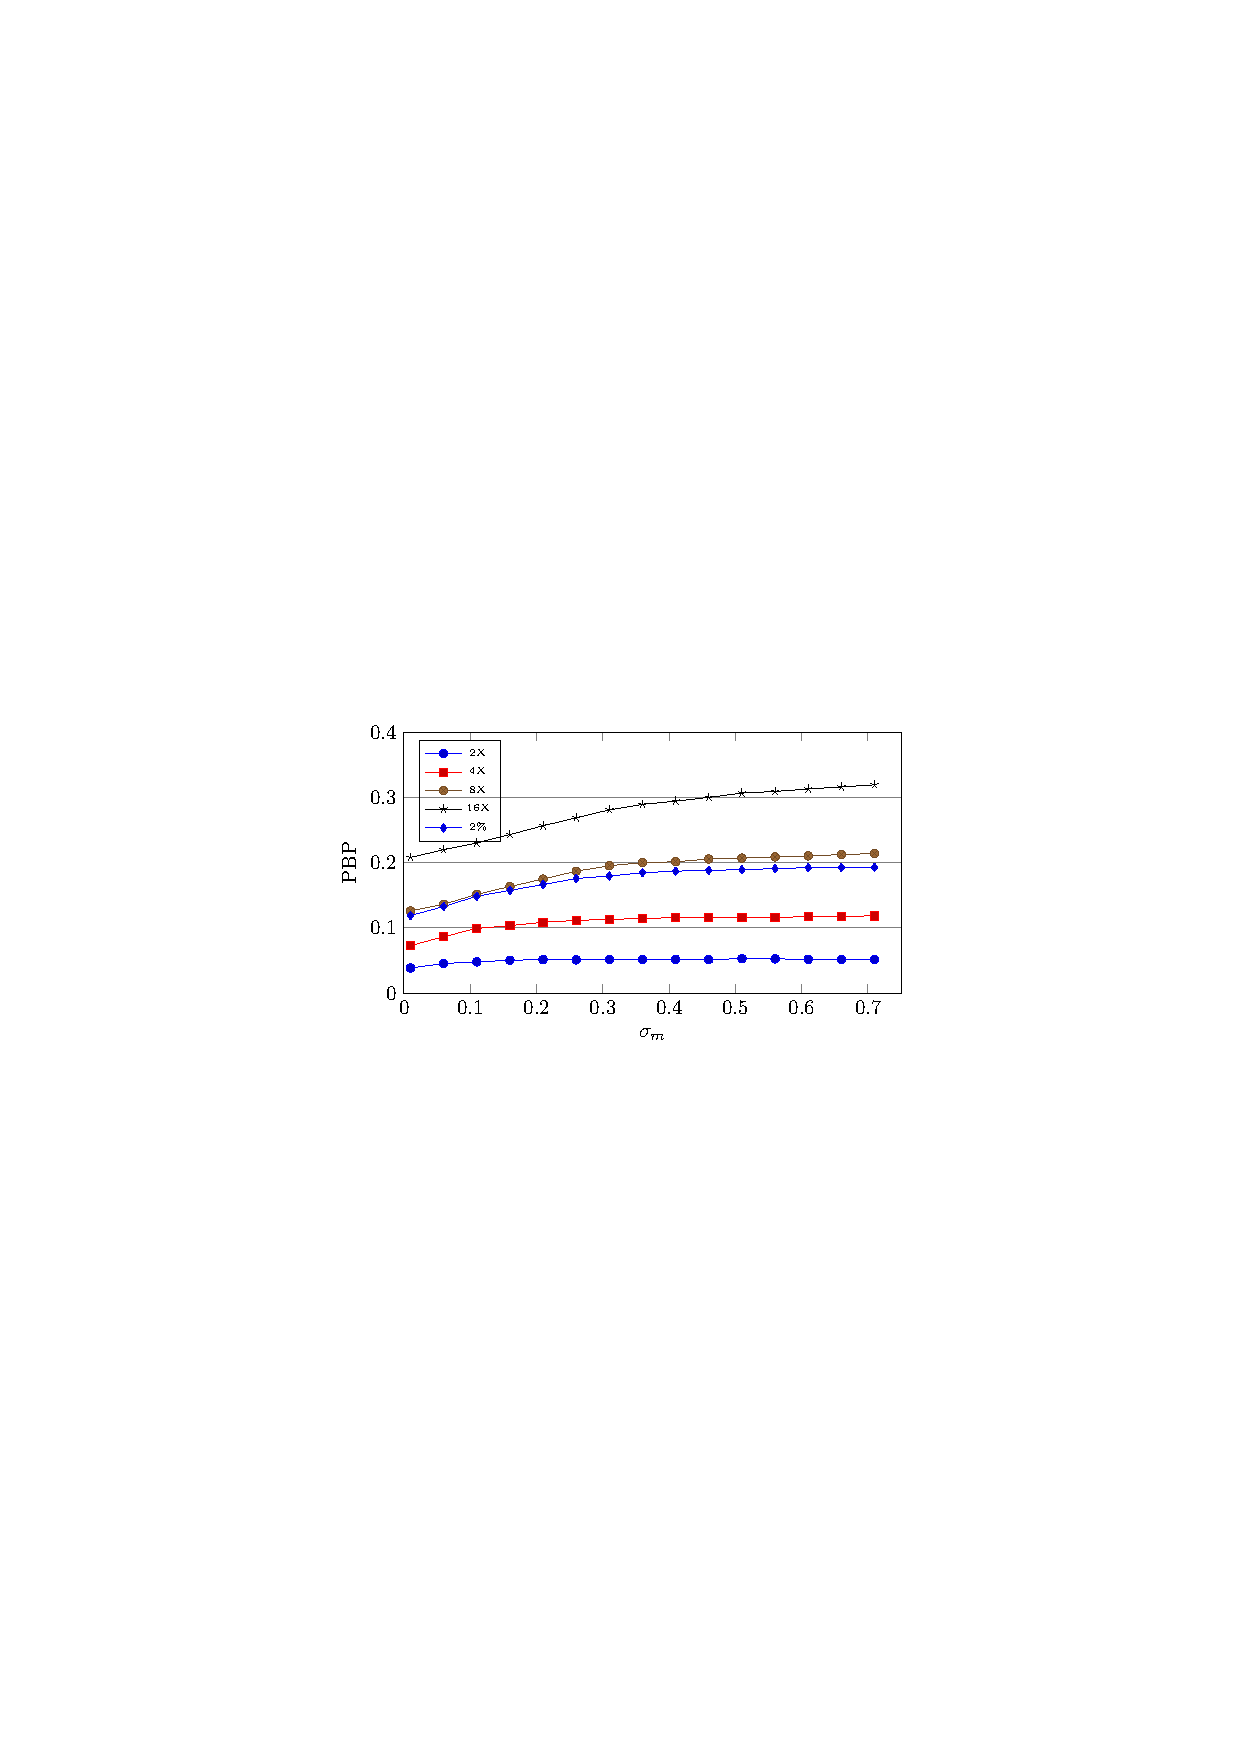
\includegraphics[width=\linewidth]{PBP1.pdf}
    \captionsetup{skip=0pt}
    \caption{Discontinuous regions}
    \label{fig}
\end{subfigure}%
\hspace{0.1\linewidth}
\begin{subfigure}[b]{0.4\linewidth}
    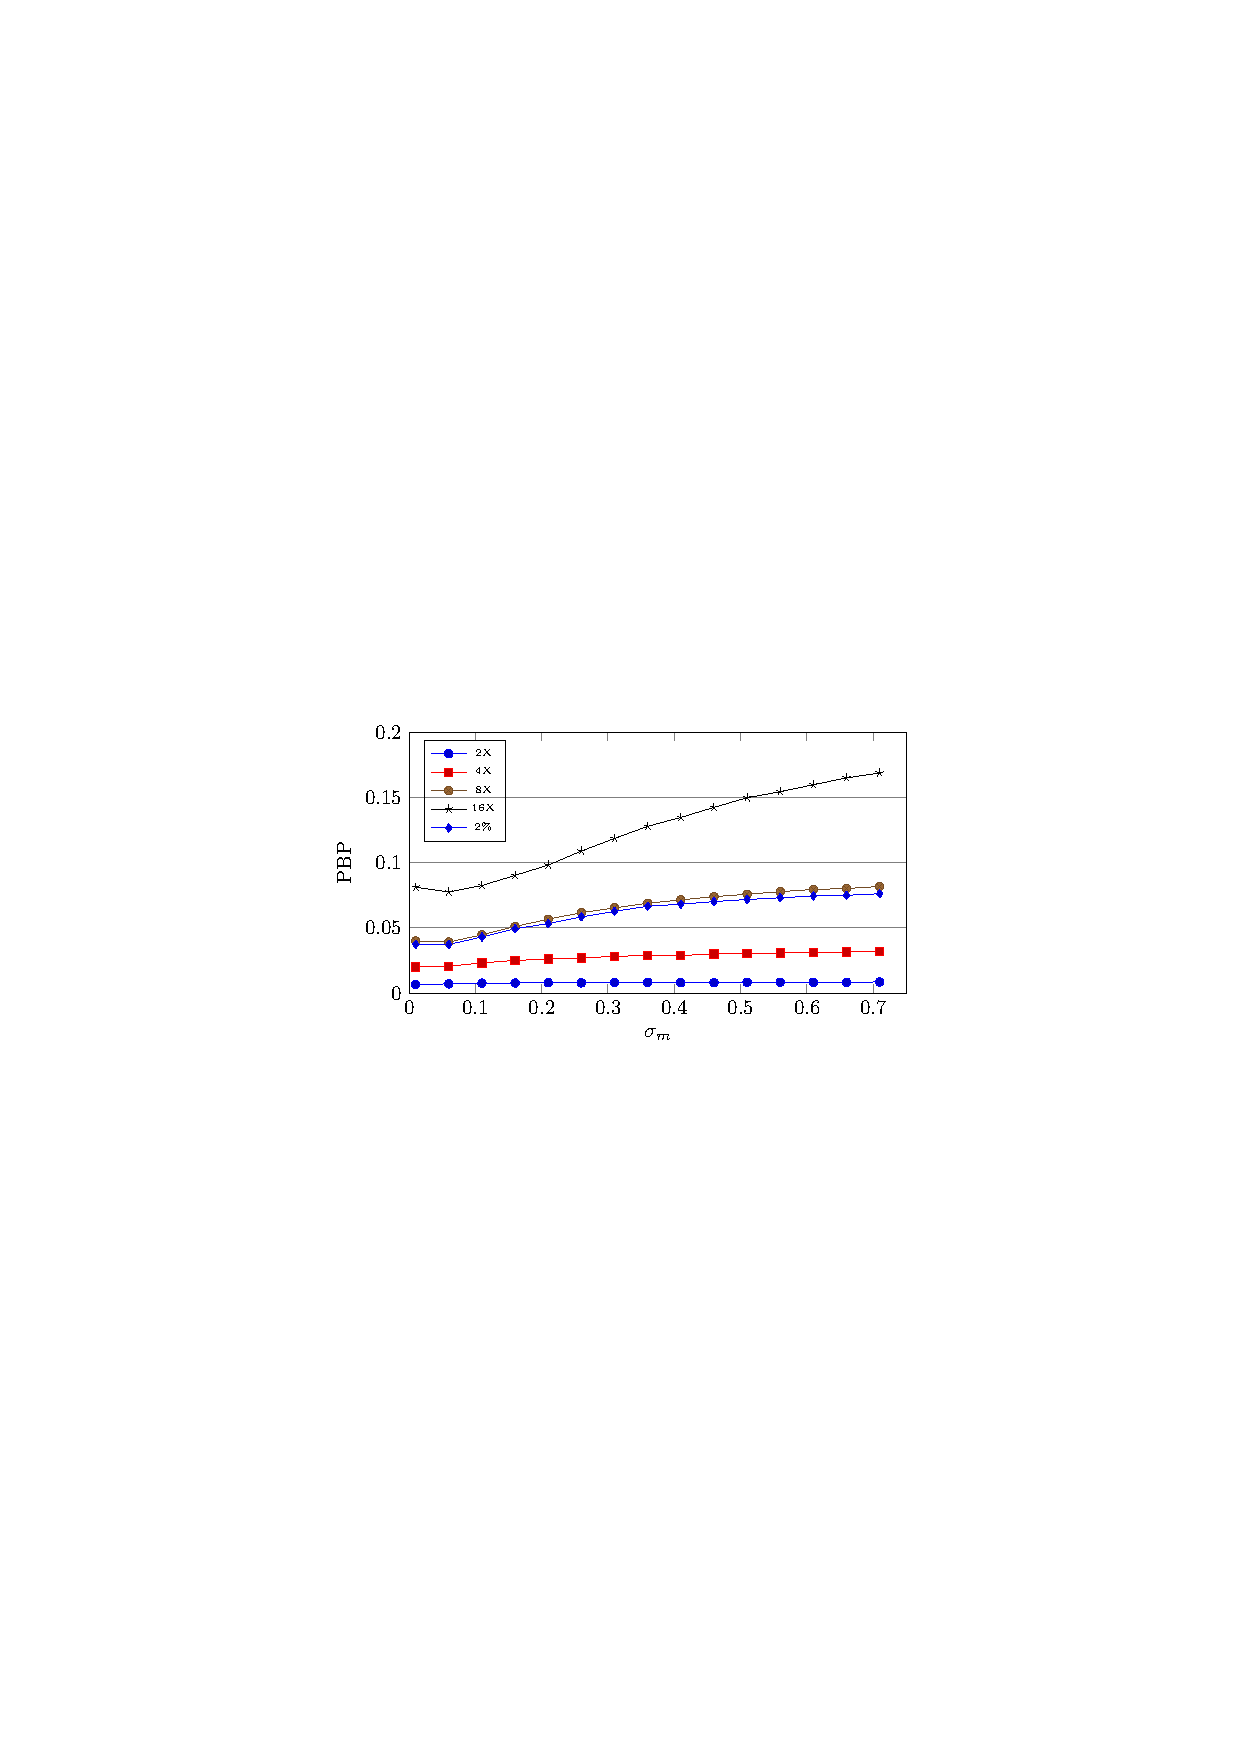
\includegraphics[width=\linewidth]{PBP2.pdf}
    \captionsetup{skip=0pt}
    \caption{Continuous areas}
    \label{fig:} %% label for first subfigure
 \end{subfigure}%
%\vspace{-0.3cm}
\caption{ PBP performance curves of discontinuous regions and continuous areas are shown as a function of $\sigma_m$. The proposed algorithm renders good performance for a wide range of $\sigma_m$ under 2X, 4X, 8X, 16X upsampling rates and 2\% random missing inpainting.
}
\label{fig:sensitivity}
\vspace{-0.2cm}
\end{figure}


\subsection{Parameter Sensitivity \& Computation Analysis}
\label{sec:sensitivity}

The parameter setting of our method is simpler than other depth upsampling methods because the only parameter is $\sigma_m$ that adjusts the similarity of coupled nodes. With varying $\sigma_m$, we record the PBP of our method to draw the performance curve of PBP and report the statistical data in Fig.~\ref{fig:sensitivity}. The figure exhibits that the performance of our algorithm at the discontinuous regions and continuous areas are rather robust in a wide range of $\sigma_m$, therefore we do not need to fine tweak the scale factor $\sigma_m$ for pursuing stable results.

We use a $690 \times 560$ image to test the efficiency of our method. Our method's computational time is stable at 8 fps for 2\% random missing inpainting and 2x, 4x, 8x upsampling. In contrast to the fastest upsampling method~\cite{Liu2013} which achieves 0.03 fps for exact method and 3 fps for approximation approach, our algorithm outperforms it significantly.

\subsection{Comparison with Yang��s method}

This section is devoted to explain why our method is better than Yang's, since our method is derived from and similar to the method of Yang~\cite{Yang2012}. Fig.~\ref{fig:comparison1} shows the comparison results of Book. We can observe that our method keeps the sharp depth edges much better. We own this achievement to the reliable seed choosing strategy. Specifically, Yang's aggregation method does not distinguish the different pixels and thus each pixel receives the contribution of all other pixels indiscriminately. On the contrary, our method only takes advantage of reliable seeds (or the closest points in the sense of minimax distance). In this way, our method successfully rules out the negative effects of the unreliable depths that are far from the target pixels.

\begin{figure}[t]
%\vspace{-0.5cm}
\centering
\begin{subfigure}[b]{0.3\linewidth}
    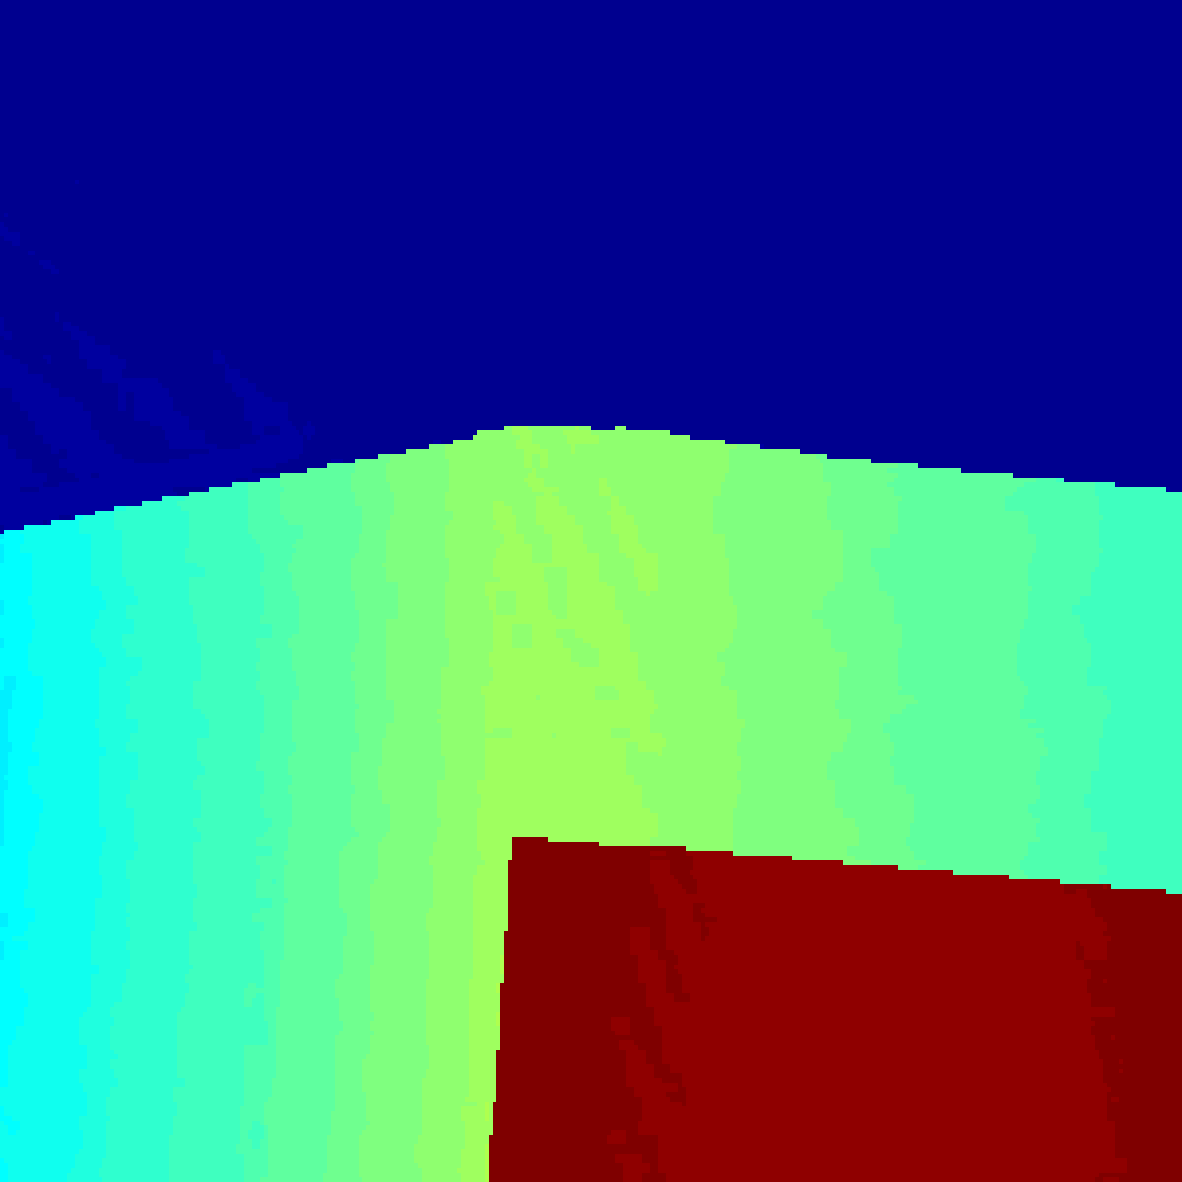
\includegraphics[ width=0.9\linewidth]{book_8X_groundtruth_color_part.png}
    \captionsetup{skip=0pt}
    \caption{Ground truth}
    \label{fig}
\end{subfigure}%
\hspace{0.005\linewidth}
\begin{subfigure}[b]{0.3\linewidth}
    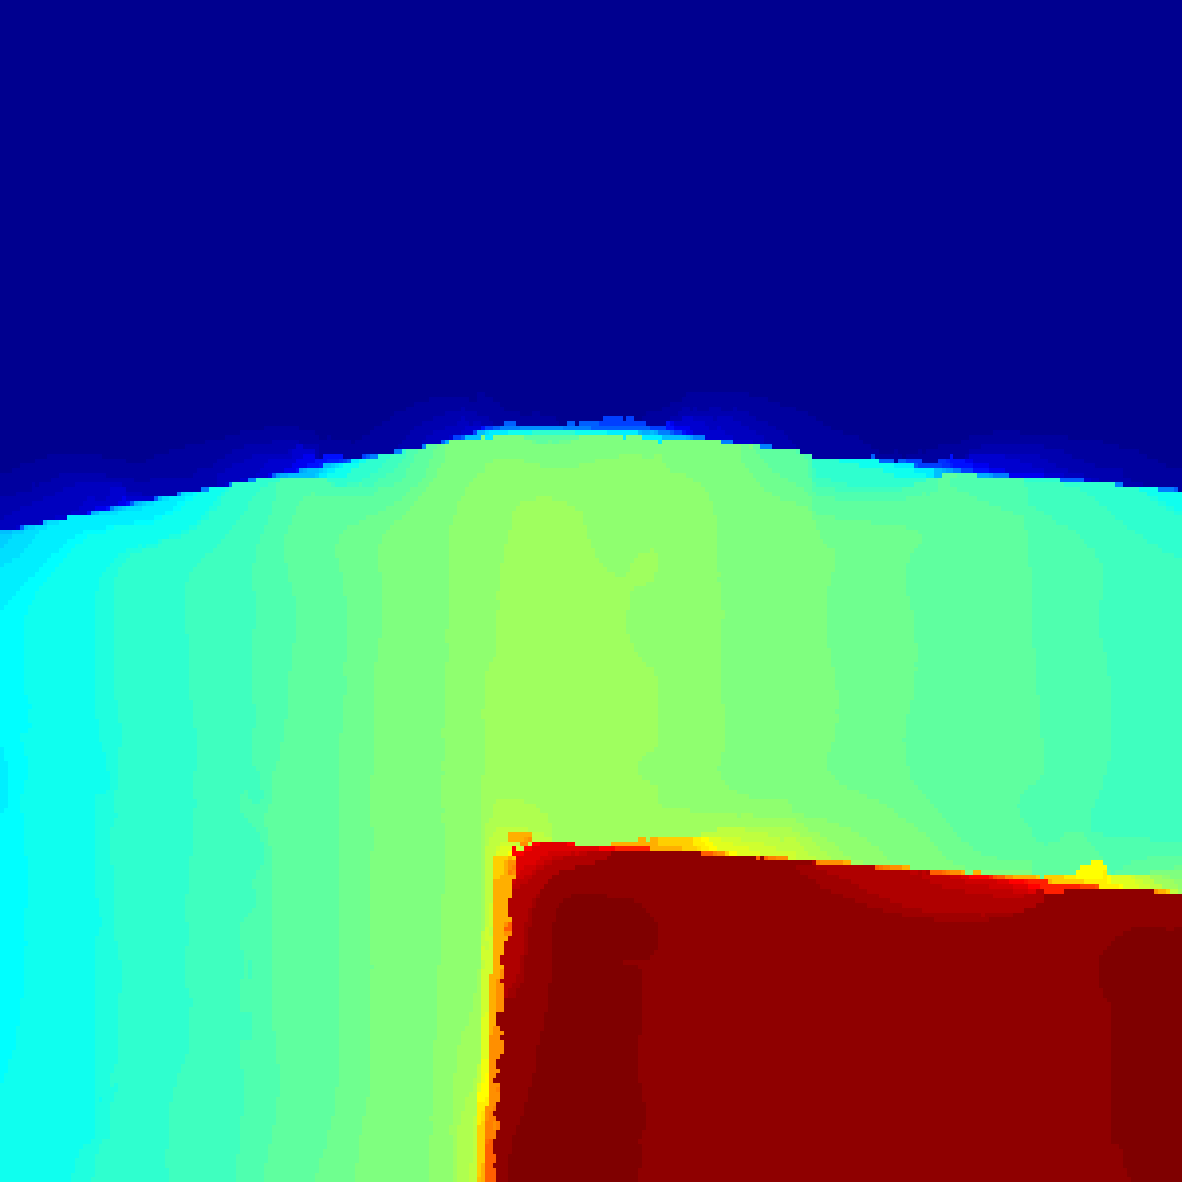
\includegraphics[width=0.9\linewidth]{book_8X_BF_color.png}
    \captionsetup{skip=0pt}
    \caption{Yang's}
    \label{fig}
\end{subfigure}%
\hspace{0.005\linewidth}
\begin{subfigure}[b]{0.3\linewidth}
    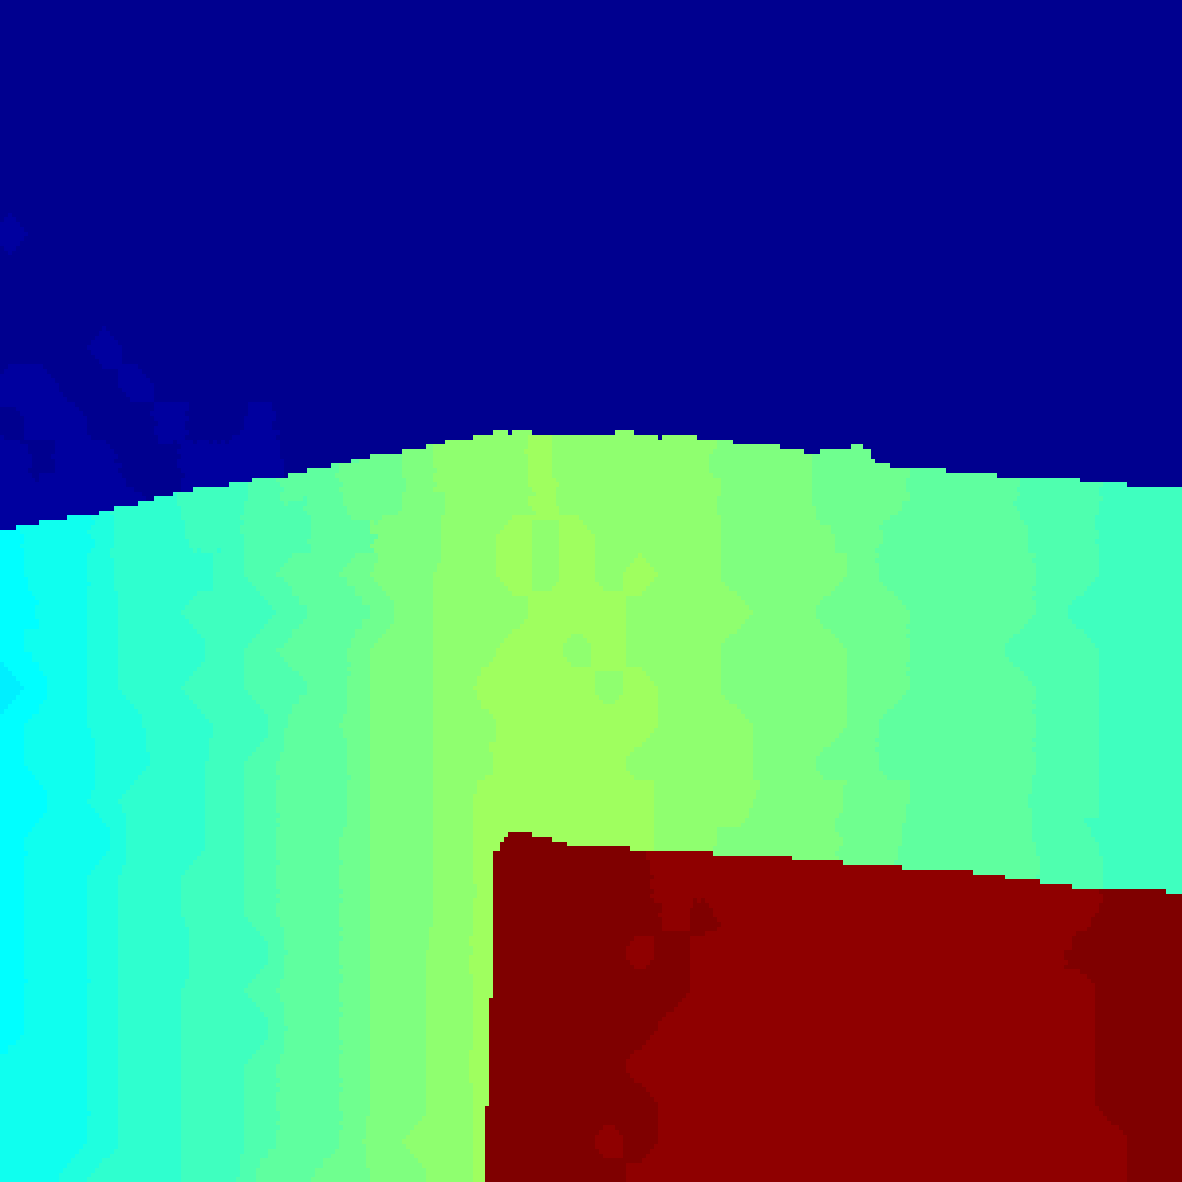
\includegraphics[width=0.9\linewidth]{book_8X_Ours_color_part.png}
    \captionsetup{skip=0pt}
    \caption{Ours}
    \label{fig}
\end{subfigure}%
\caption{Close-ups of the 8X upsampled result of book. For clarity, we visualize the image intensities using a color map. We can observes that our method can keep the sharp depth edges satisfactorily.}
\label{fig:comparison1}
\vspace{-0.2cm}
\end{figure}


\IEEEtriggeratref{13}


\bibliographystyle{IEEEtran}
\bibliography{paper}

\end{document} 